\documentclass[12pt,a4paper]{article}
\usepackage[utf8]{inputenc}
\usepackage[catalan]{babel}
\usepackage{graphicx}
\usepackage{geometry}
\usepackage{fancyhdr}
\usepackage{tabularx}
\usepackage{lastpage}
\usepackage{enumitem}
\usepackage{amsmath}
\usepackage{float}
\usepackage{hyperref}

% 1. MARGES I CAPÇALERA
\geometry{top=4cm, bottom=3cm, left=2cm, right=2cm, headheight=2.5cm}

\pagestyle{fancy}
\fancyhf{}
\fancyhead[L]{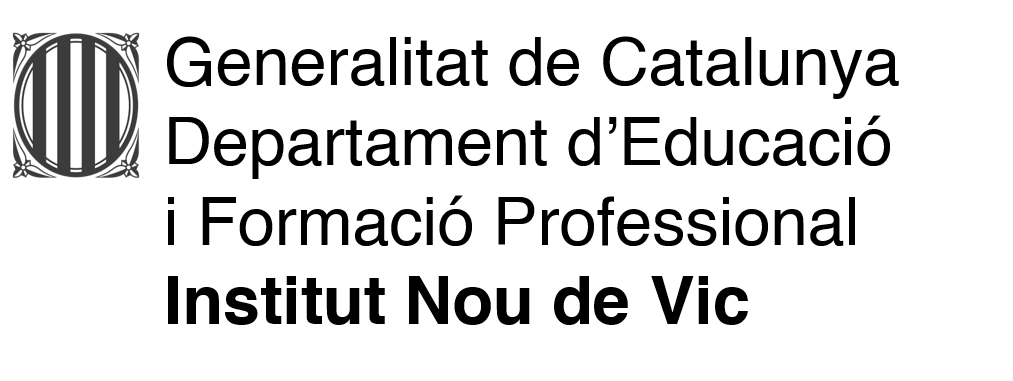
\includegraphics[height=1.8cm]{Logo_Departament.png}} 
\fancyhead[R]{
\includegraphics[height=1.8cm]{Logo_Institut.png}}

\fancyfoot[L]{}
\fancyfoot[C]{Pàgina \thepage\ de \pageref{LastPage}}
\fancyfoot[R]{}

\renewcommand{\headrulewidth}{0.4pt}

\begin{document}

% --- CAPÇALERA D'IDENTIFICACIÓ ---
\begingroup
\renewcommand{\arraystretch}{2.2}
\begin{tabularx}{\textwidth}{|X|p{4cm}|}
    \hline
    \textbf{Nom i cognoms:} & \textbf{Grup:} \\ \hline
    \textbf{Activitat:} Vectors i Geometria & \textbf{Data:} \\ \hline
\end{tabularx}
\endgroup

\vspace{0.8cm}

\begin{center}
    {\Large \textbf{ACTIVITATS: VECTORS EN EL PLA}}
\end{center}

\vspace{0.5cm}

% ---------------------------------------------------------
% EXERCICI 42: PARAL·LELOGRAM
% ---------------------------------------------------------

\section{Exercici 42: Paral·lelogram i intersecció diagonals}

\subsection*{Enunciat}
Sabem que els punts $A(1, 2)$, $B(3, 5)$ i $C(7, 4)$ són tres vèrtexs consecutius d'un paral·lelogram. 
\begin{enumerate}
    \item Calcula les coordenades del quart vèrtex $D$.
    \item Calcula el punt $M$ on es tallen les dues diagonals.
\end{enumerate}

\vspace{0.3cm}
\noindent \textbf{Recurs interactiu:} \url{https://www.geogebra.org/calculator/hnf7m5as}

\subsection*{Resolució}

\subsubsection*{1. Representació dels punts coneguts}
Primer situem els tres punts donats al pla.

\begin{center}
    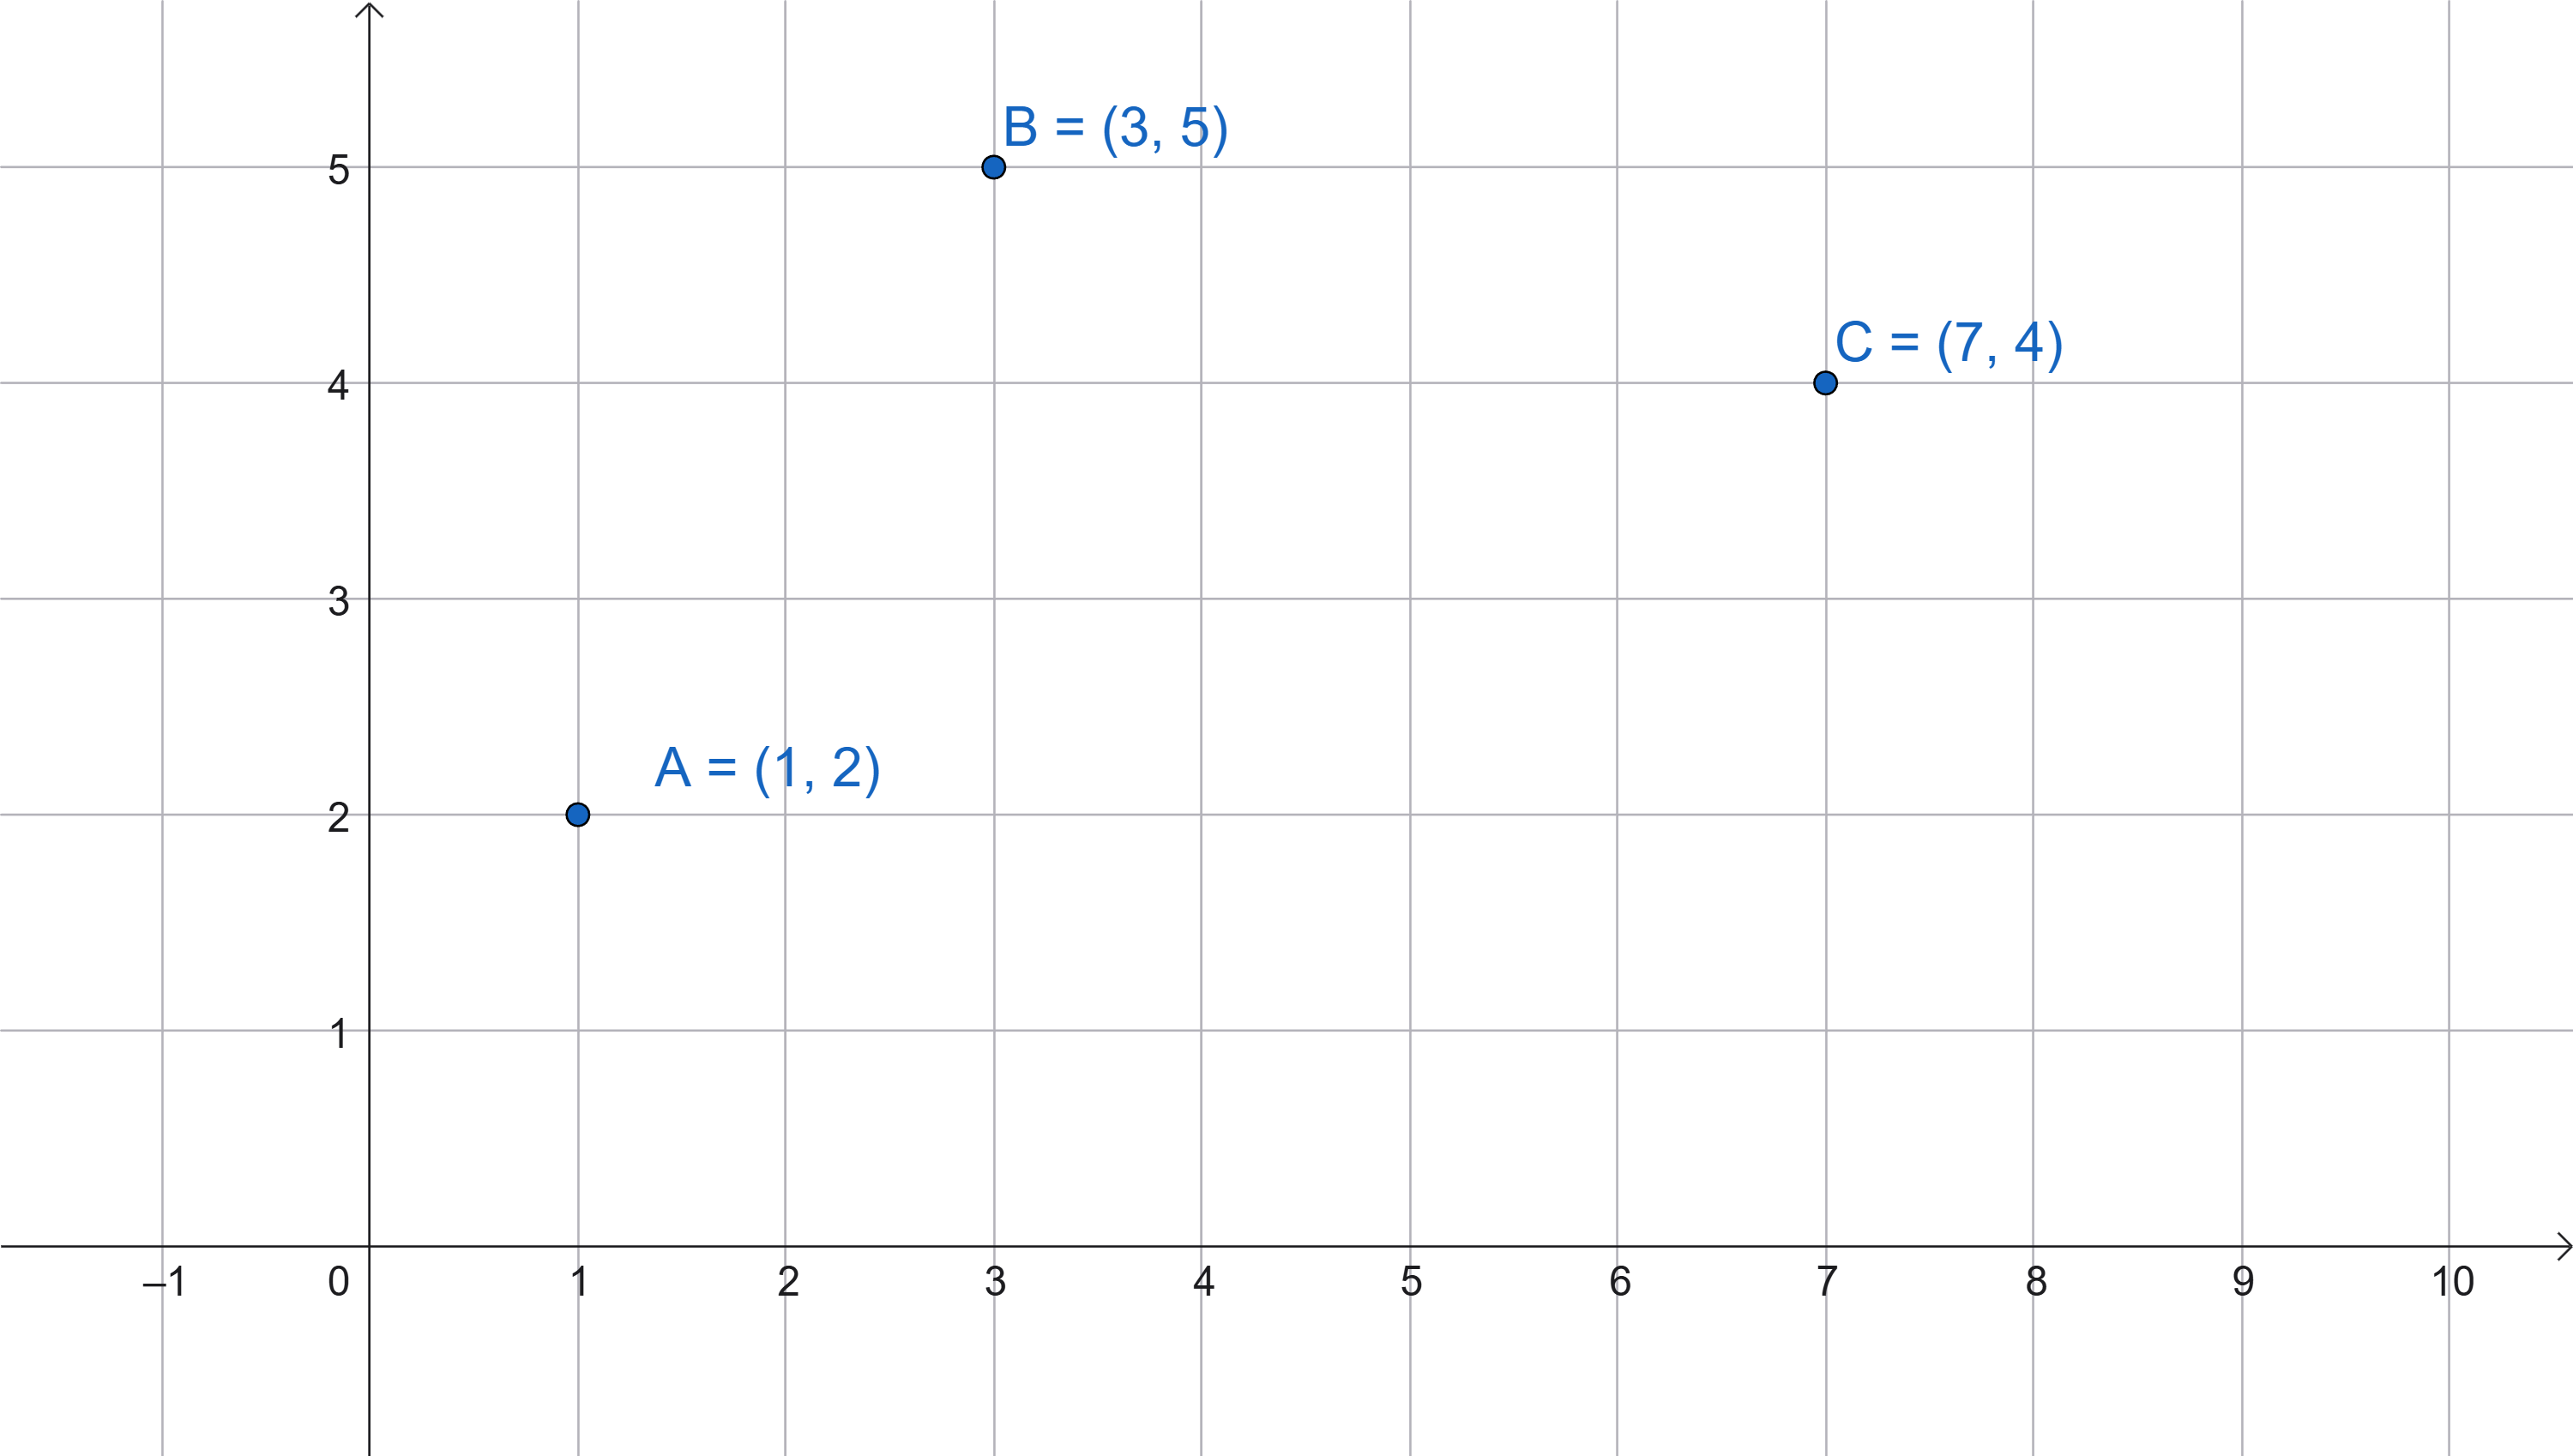
\includegraphics[width=10cm]{Vectors - 42 - Paral·lelogram - Intersecció diagonals_1.png}
\end{center}

\subsubsection*{2. Càlcul del quart vèrtex ($D$)}
En un paral·lelogram, els costats oposats són paral·lels i iguals. Això implica que el vector $\vec{BA}$ és equipol·lent al vector $\vec{CD}$.

Primer calculem el vector $\vec{BA}$:
$$ \vec{BA} = A - B = (1 - 3, 2 - 5) = (-2, -3) $$

Com que $\vec{CD} = \vec{BA}$, per trobar el punt $D$ només hem de sumar aquest vector al punt $C$:
$$ D = C + \vec{BA} $$
$$ D = (7, 4) + (-2, -3) $$
$$ D = (7 - 2, 4 - 3) = (5, 1) $$

El quart vèrtex és \textbf{$D(5, 1)$}.

\begin{center}
    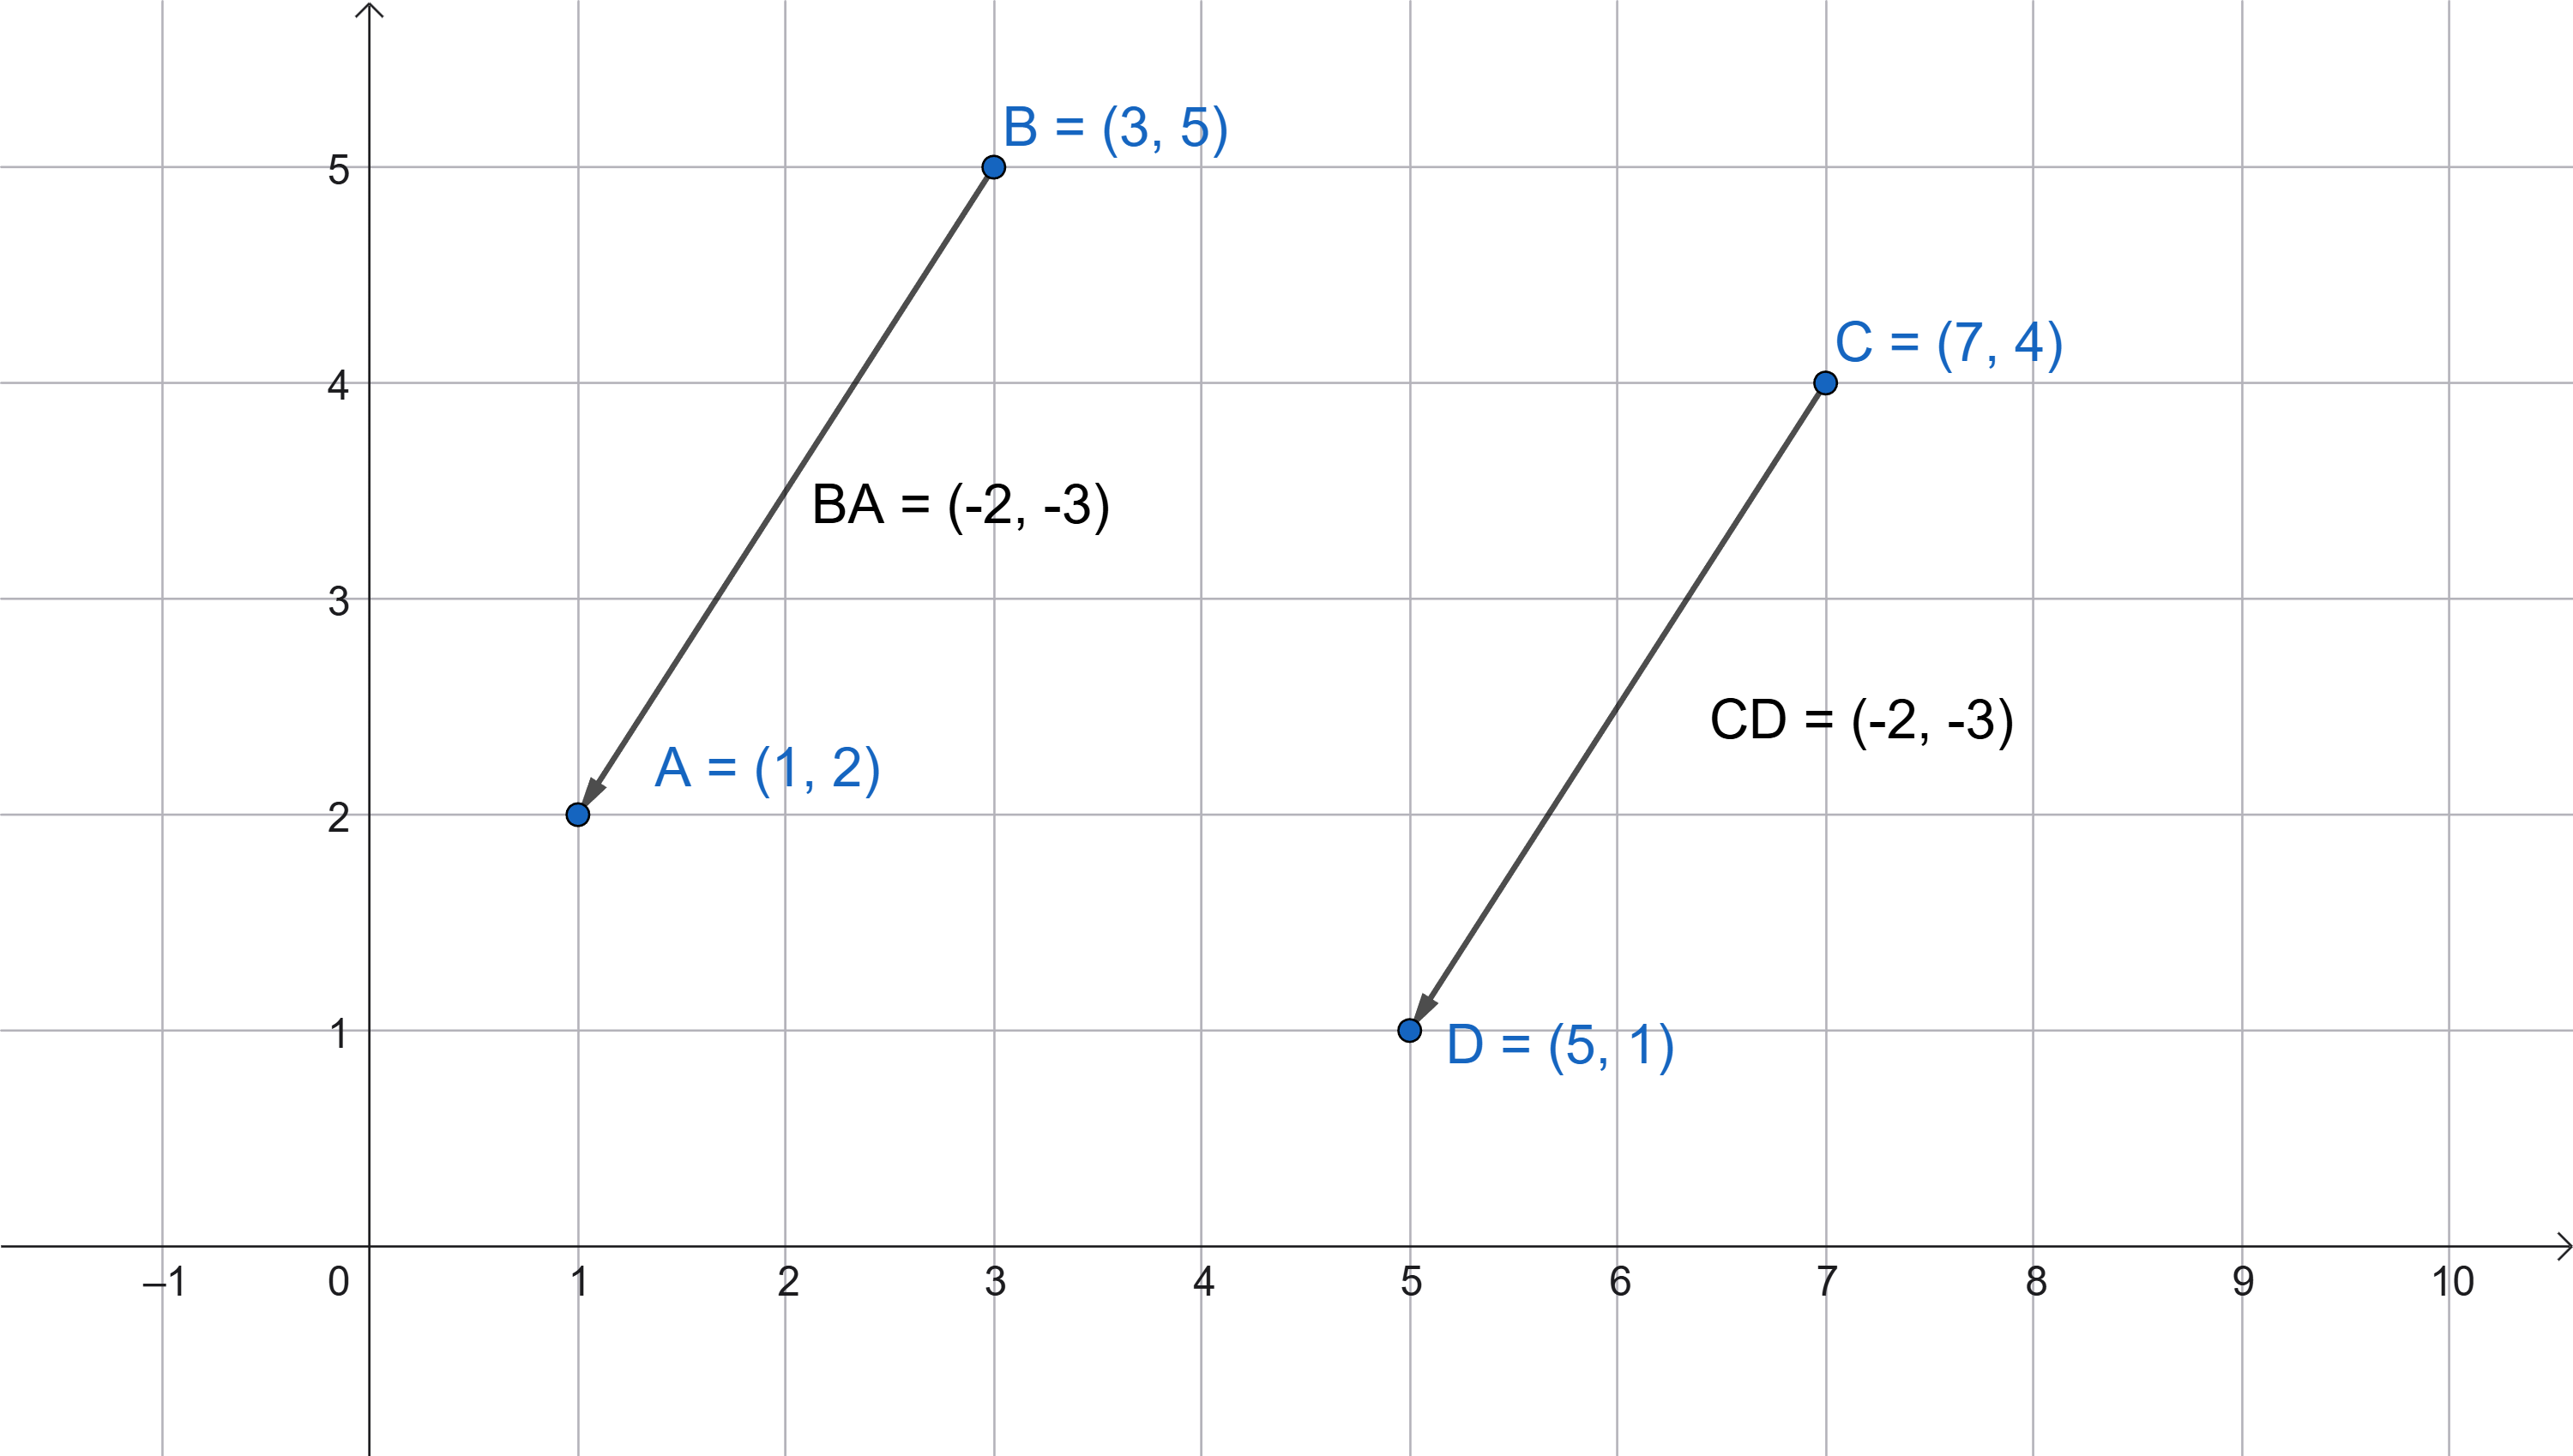
\includegraphics[width=10cm]{Vectors - 42 - Paral·lelogram - Intersecció diagonals_3.png}
\end{center}

\subsubsection*{3. Càlcul de la diagonal $BD$}
Les diagonals d'un paral·lelogram es tallen en el seu punt mig. Per trobar la intersecció ($M$), calcularem el punt mig de la diagonal $BD$. Primer trobem el vector que uneix els vèrtexs oposats:

$$ \vec{BD} = D - B = (5, 1) - (3, 5) $$
$$ \vec{BD} = (5 - 3, 1 - 5) = (2, -4) $$

\begin{center}
    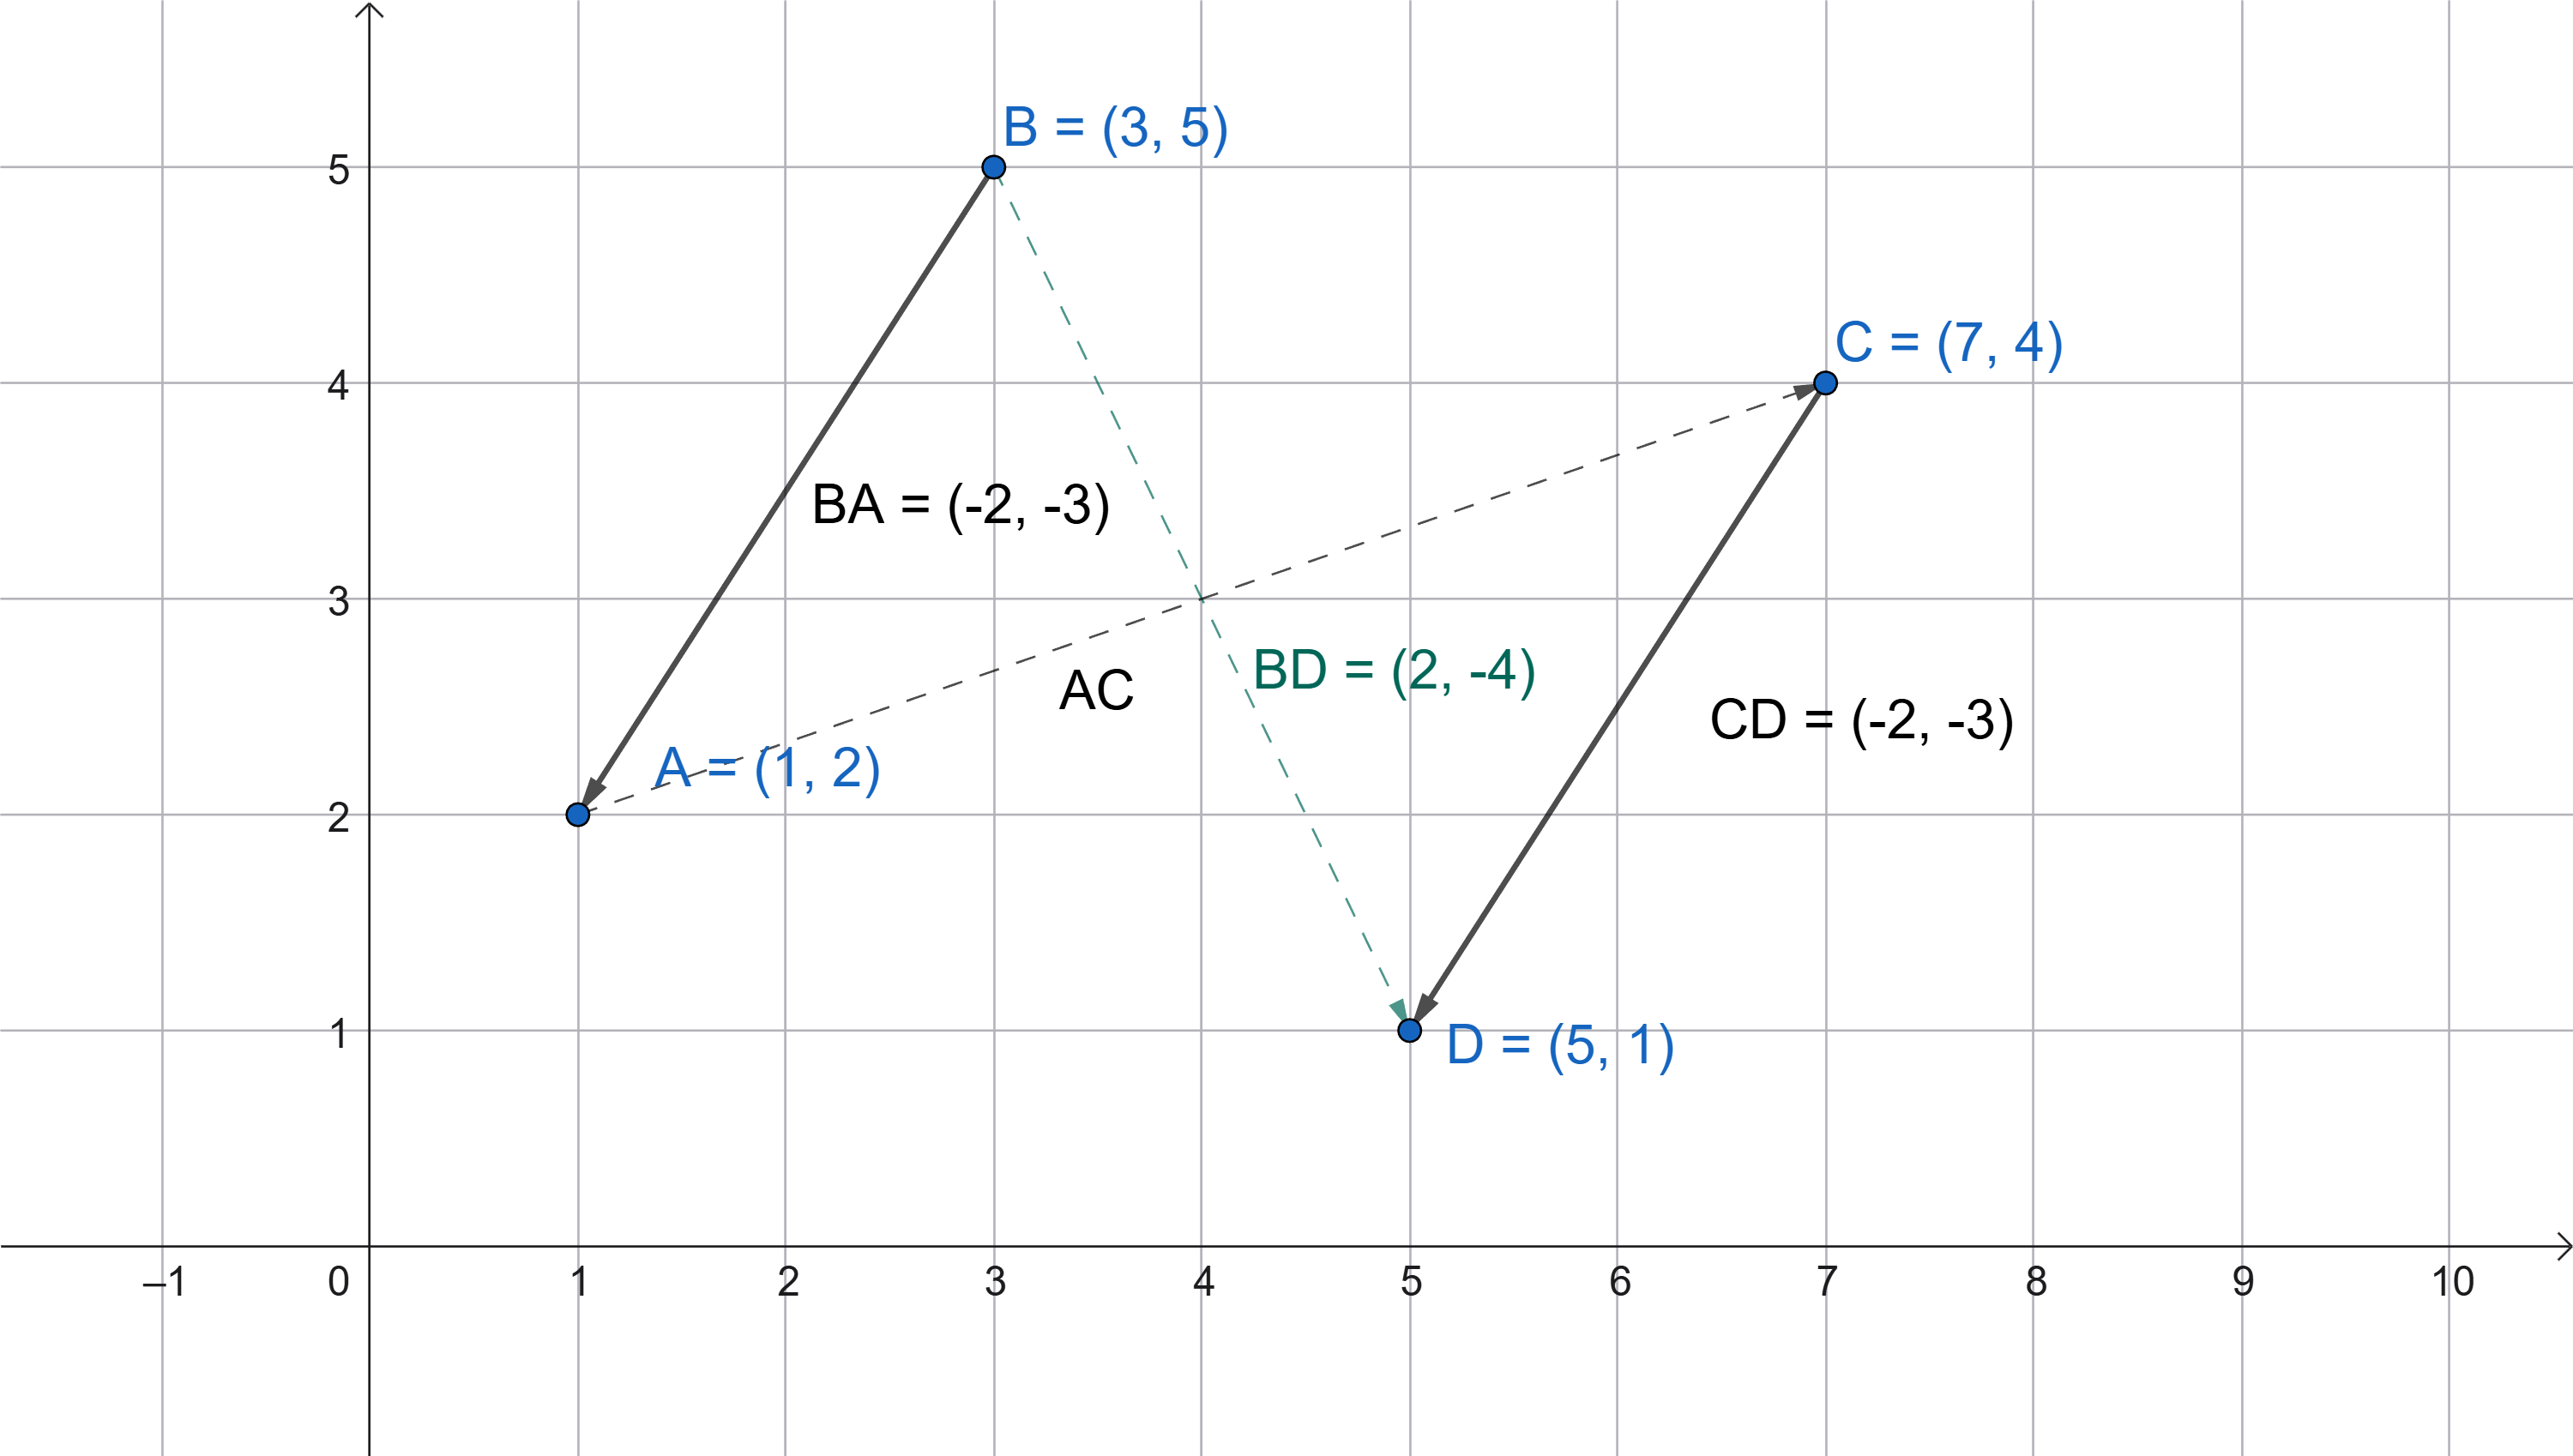
\includegraphics[width=10cm]{Vectors - 42 - Paral·lelogram - Intersecció diagonals_4.png}
\end{center}

\subsubsection*{4. Càlcul del punt mig de la diagonal ($M$)}
El punt de tall $M$ es troba sumant la meitat del vector $\vec{BD}$ al punt d'origen $B$.

Calculem la meitat del vector:
$$ \frac{1}{2}\vec{BD} = \frac{1}{2} \cdot (2, -4) = (1, -2) $$

Finalment, trobem $M$:
$$ M = B + \frac{1}{2}\vec{BD} $$
$$ M = (3, 5) + (1, -2) $$
$$ M = (3 + 1, 5 - 2) = (4, 3) $$

El punt d'intersecció de les diagonals és \textbf{$M(4, 3)$}.

\begin{center}
    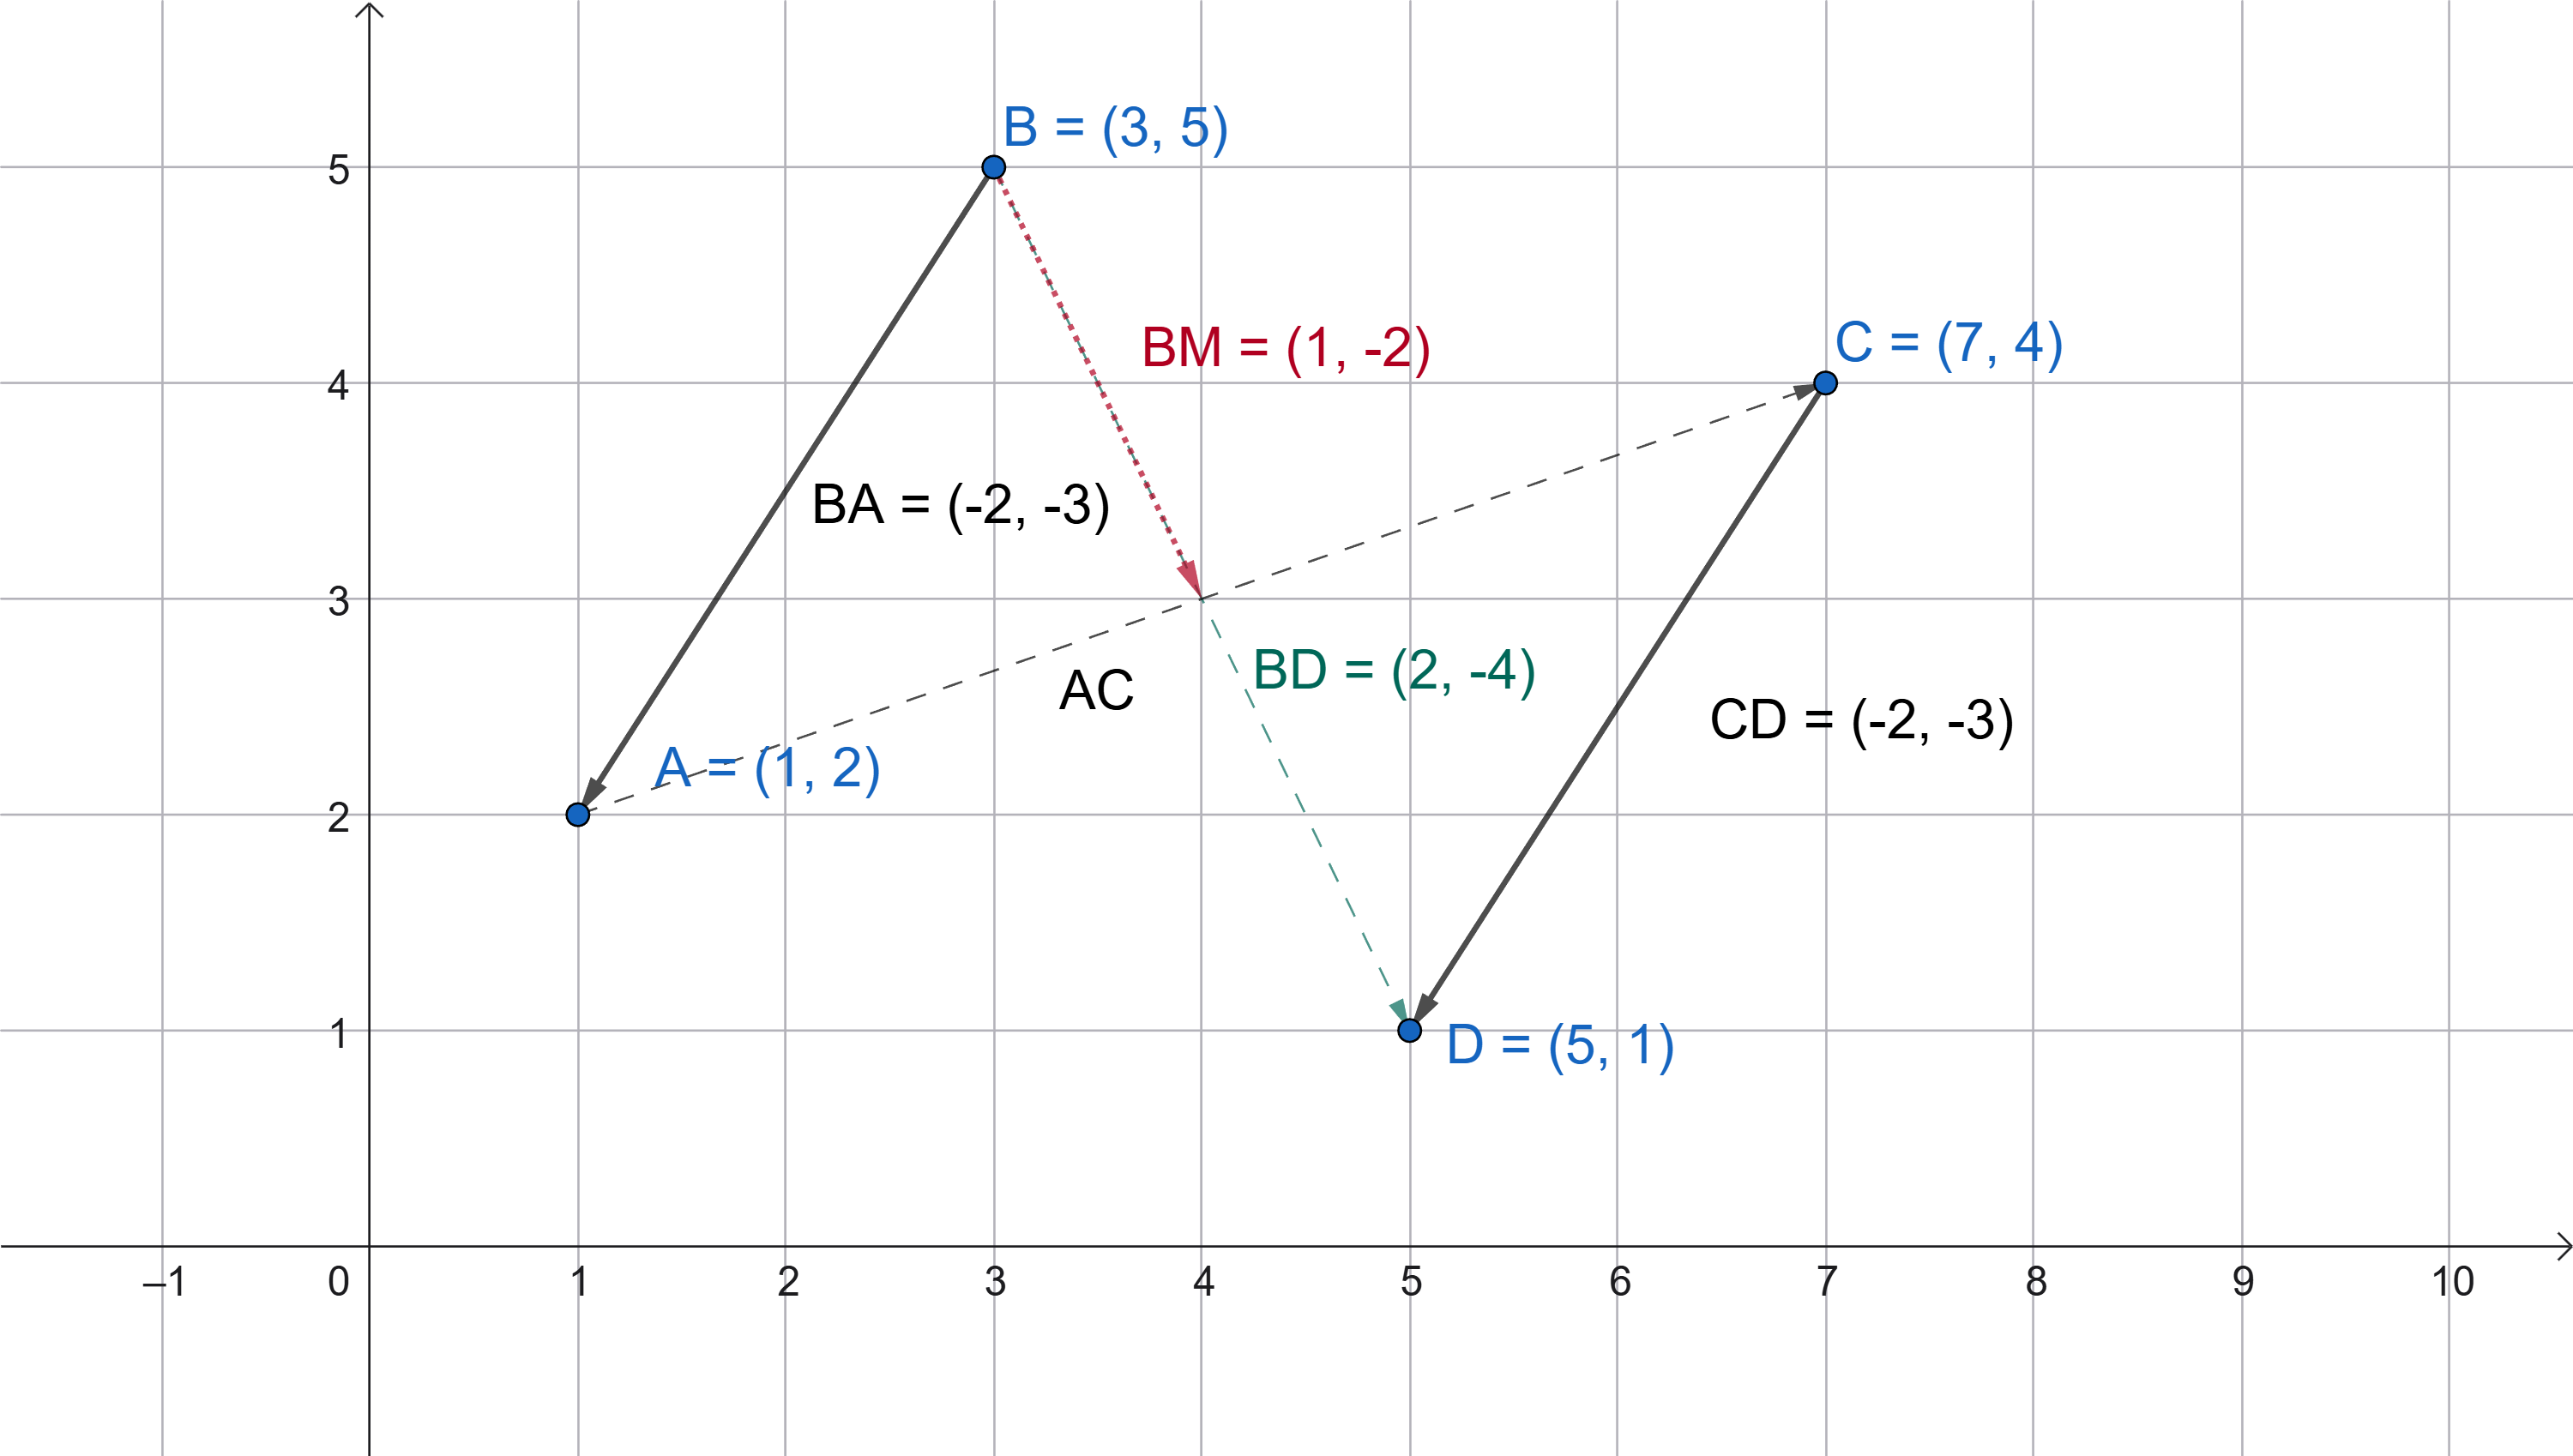
\includegraphics[width=10cm]{Vectors - 42 - Paral·lelogram - Intersecció diagonals_5.png}
\end{center}

Resultat final amb totes les dades:

\begin{center}
    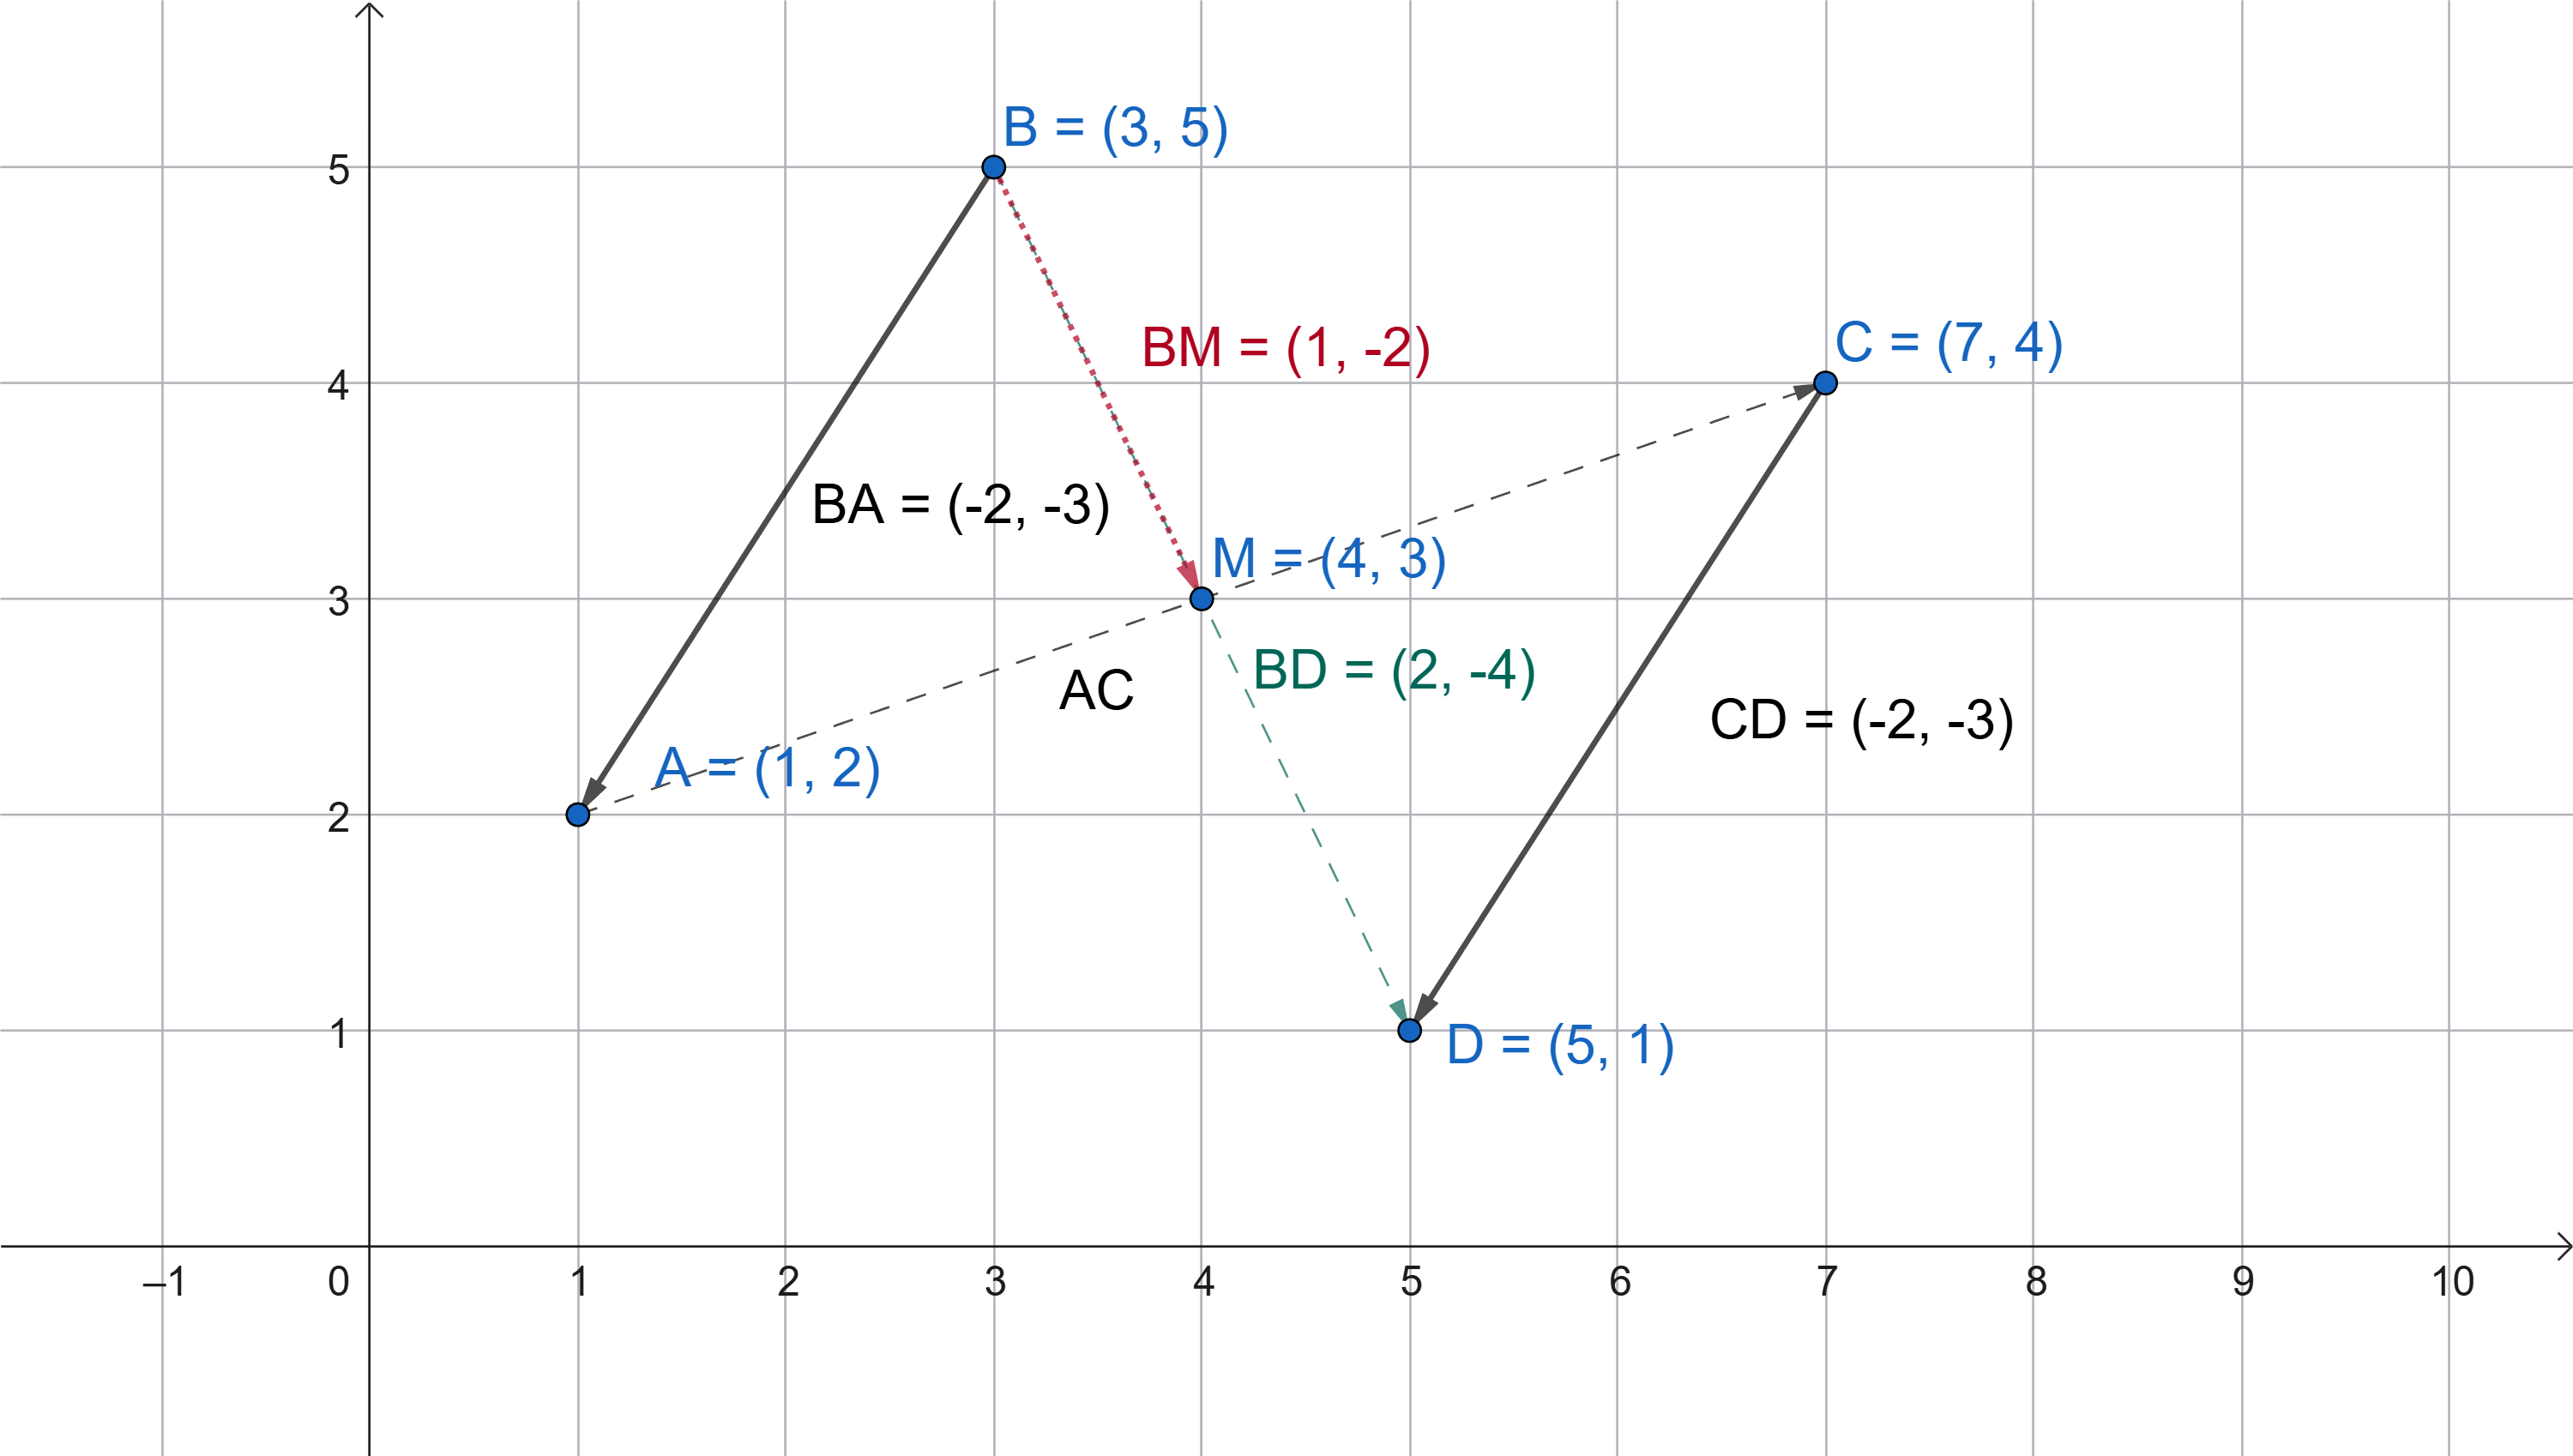
\includegraphics[width=10cm]{Vectors - 42 - Paral·lelogram - Intersecció diagonals_6.png}
\end{center}

\newpage

% ---------------------------------------------------------
% EXERCICI 44: DIVISIÓ DE SEGMENT
% ---------------------------------------------------------

\section{Exercici 44: Divisió d'un segment en tres parts}

\subsection*{Enunciat}
Donats els punts $A(-12, 6)$ i $B(0, 9)$, calcula les coordenades dels punts $A_1$ i $A_2$ que divideixen el segment $AB$ en tres parts iguals.

\vspace{0.3cm}
\noindent \textbf{Recurs interactiu:} \url{https://www.geogebra.org/calculator/krxkpdcg}

\subsection*{Resolució}

\subsubsection*{1. Representació gràfica}
Situem l'origen $A$ i l'extrem $B$.

\begin{center}
    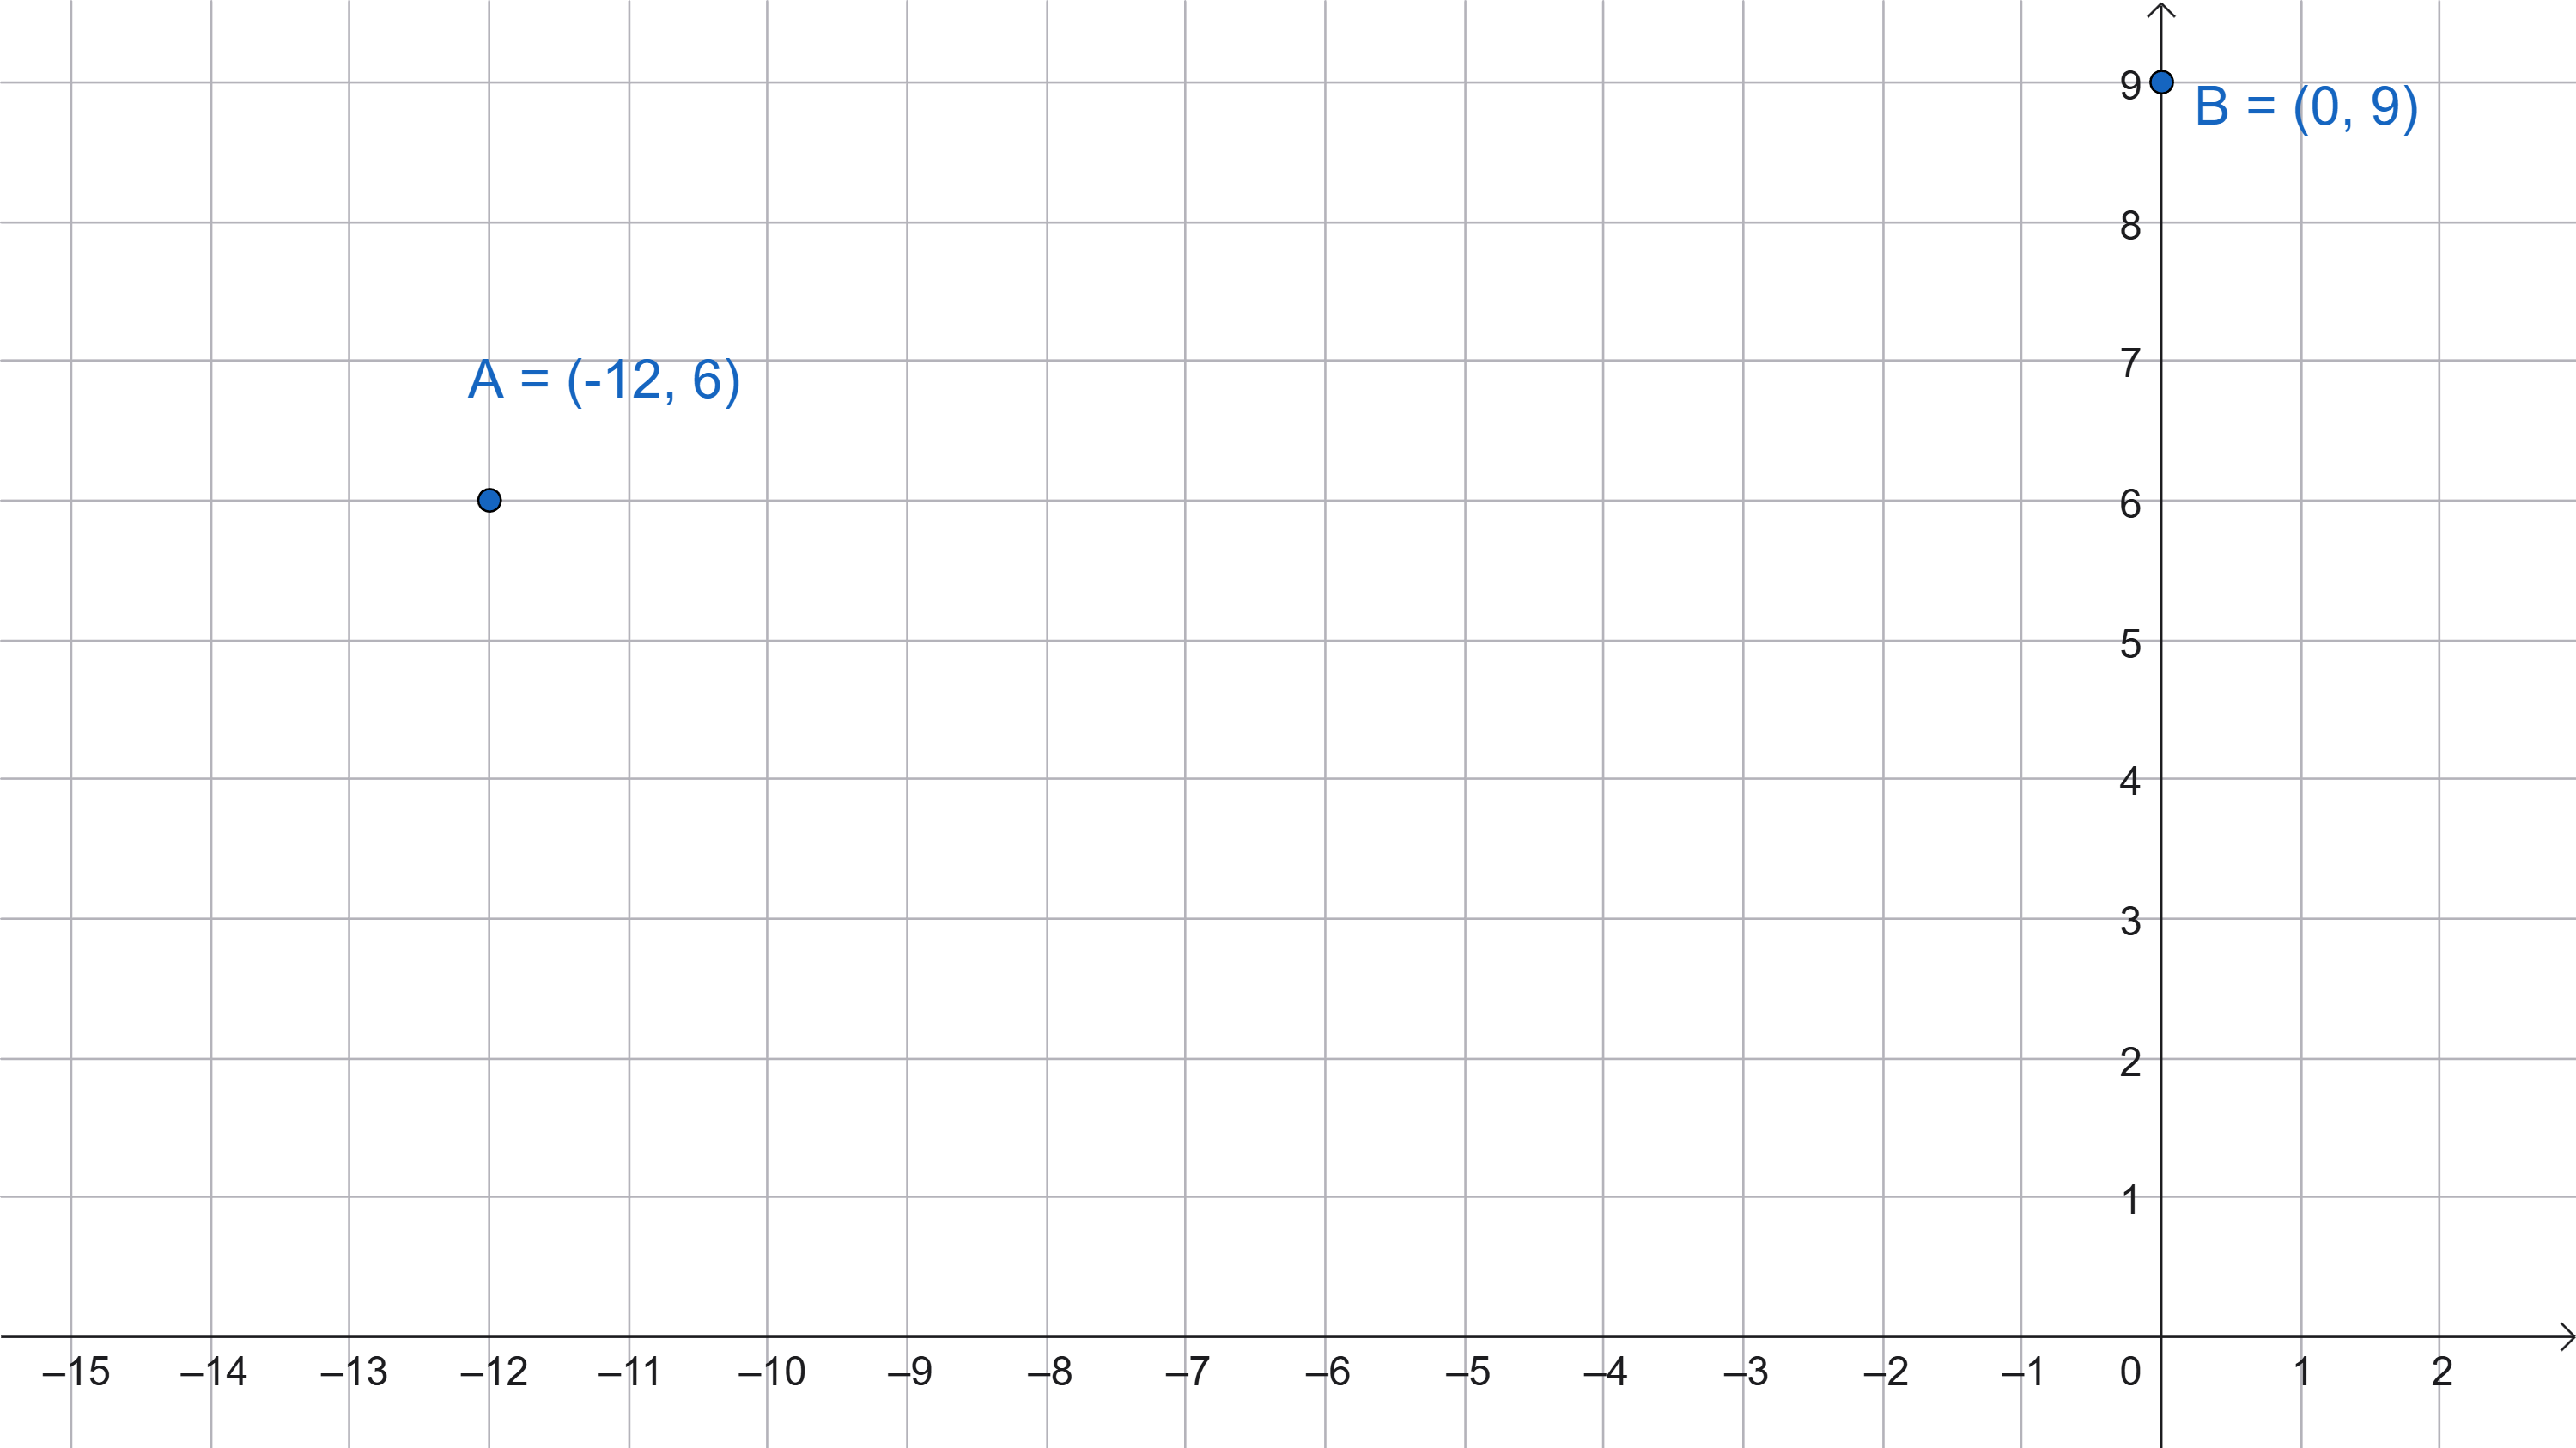
\includegraphics[width=10cm]{Vectors - 44 - Dividir punt en 3 segments_1.png}
\end{center}

\subsubsection*{2. Càlcul del vector principal $\vec{AB}$}
Calcularem el vector que va des de $A$ fins a $B$.
$$ \vec{AB} = B - A = (0 - (-12), 9 - 6) = (12, 3) $$

\begin{center}
    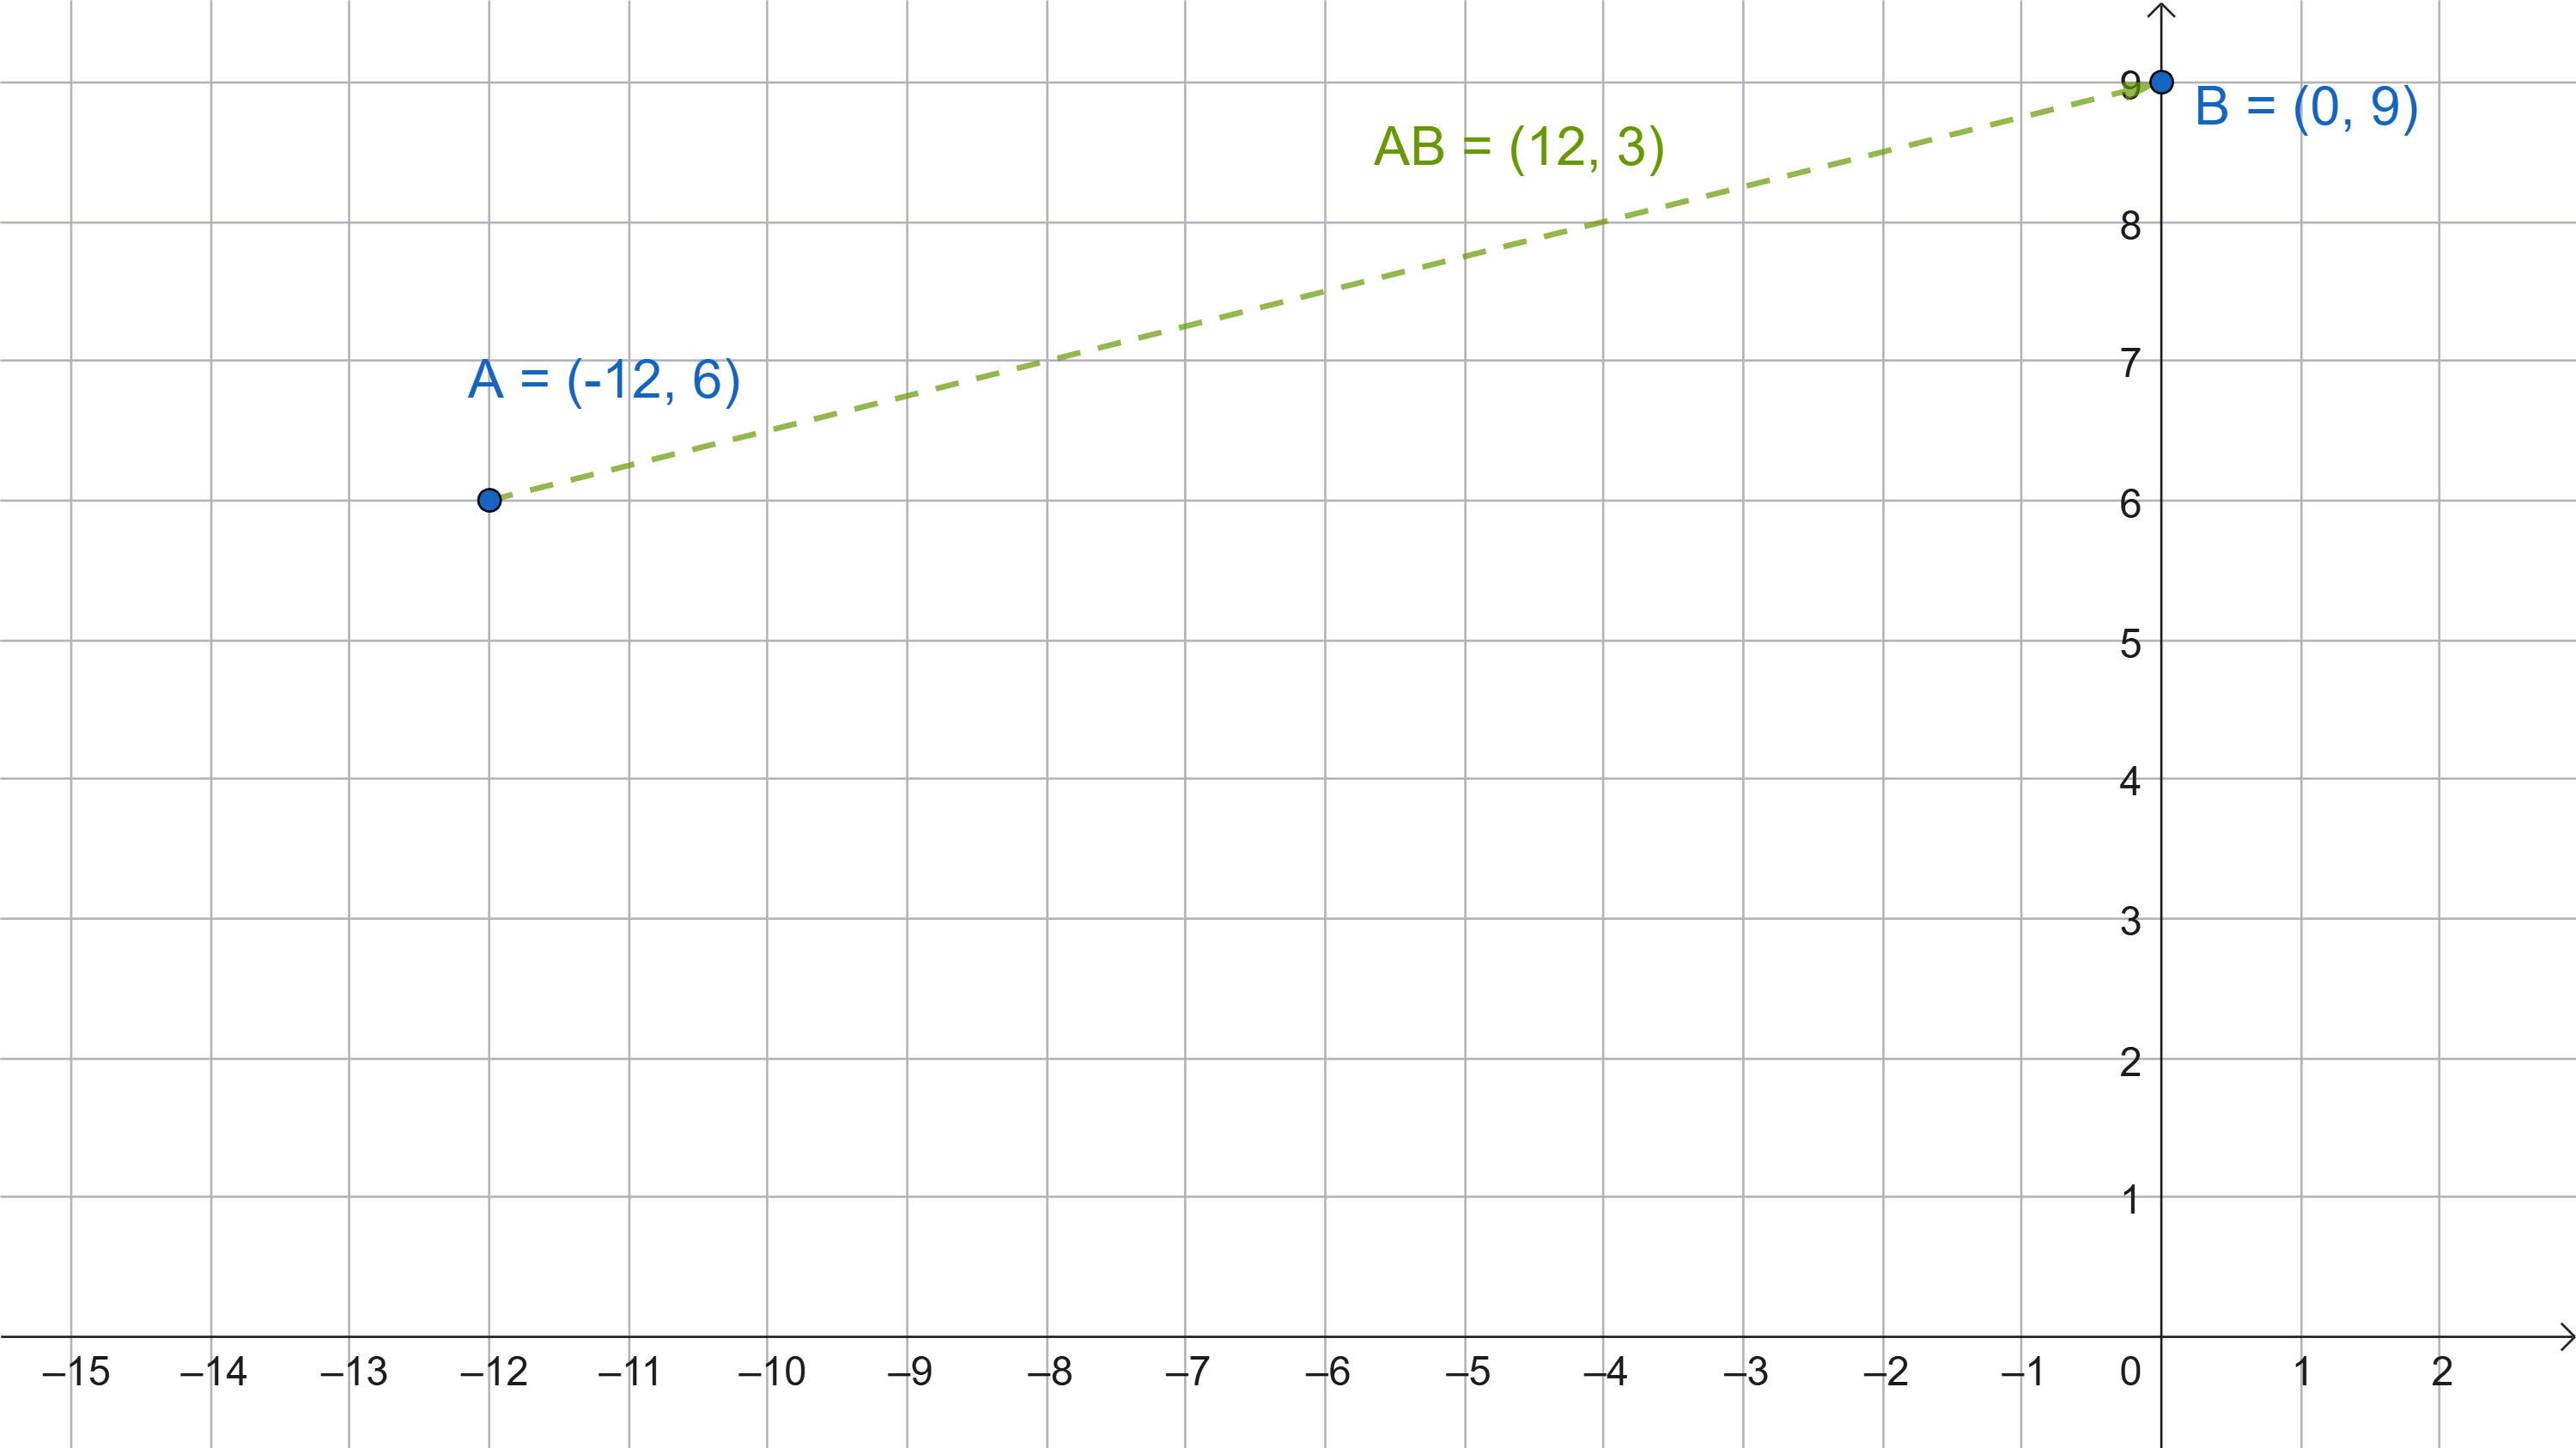
\includegraphics[width=10cm]{Vectors - 44 - Dividir punt en 3 segments_2.png}
\end{center}

\subsubsection*{3. Càlcul del vector unitari de divisió}
Com que volem dividir el segment en 3 parts, necessitem un vector que sigui exactament una tercera part de $\vec{AB}$.
$$ \vec{v} = \frac{1}{3}\vec{AB} = \frac{1}{3} \cdot (12, 3) = (4, 1) $$

\begin{center}
    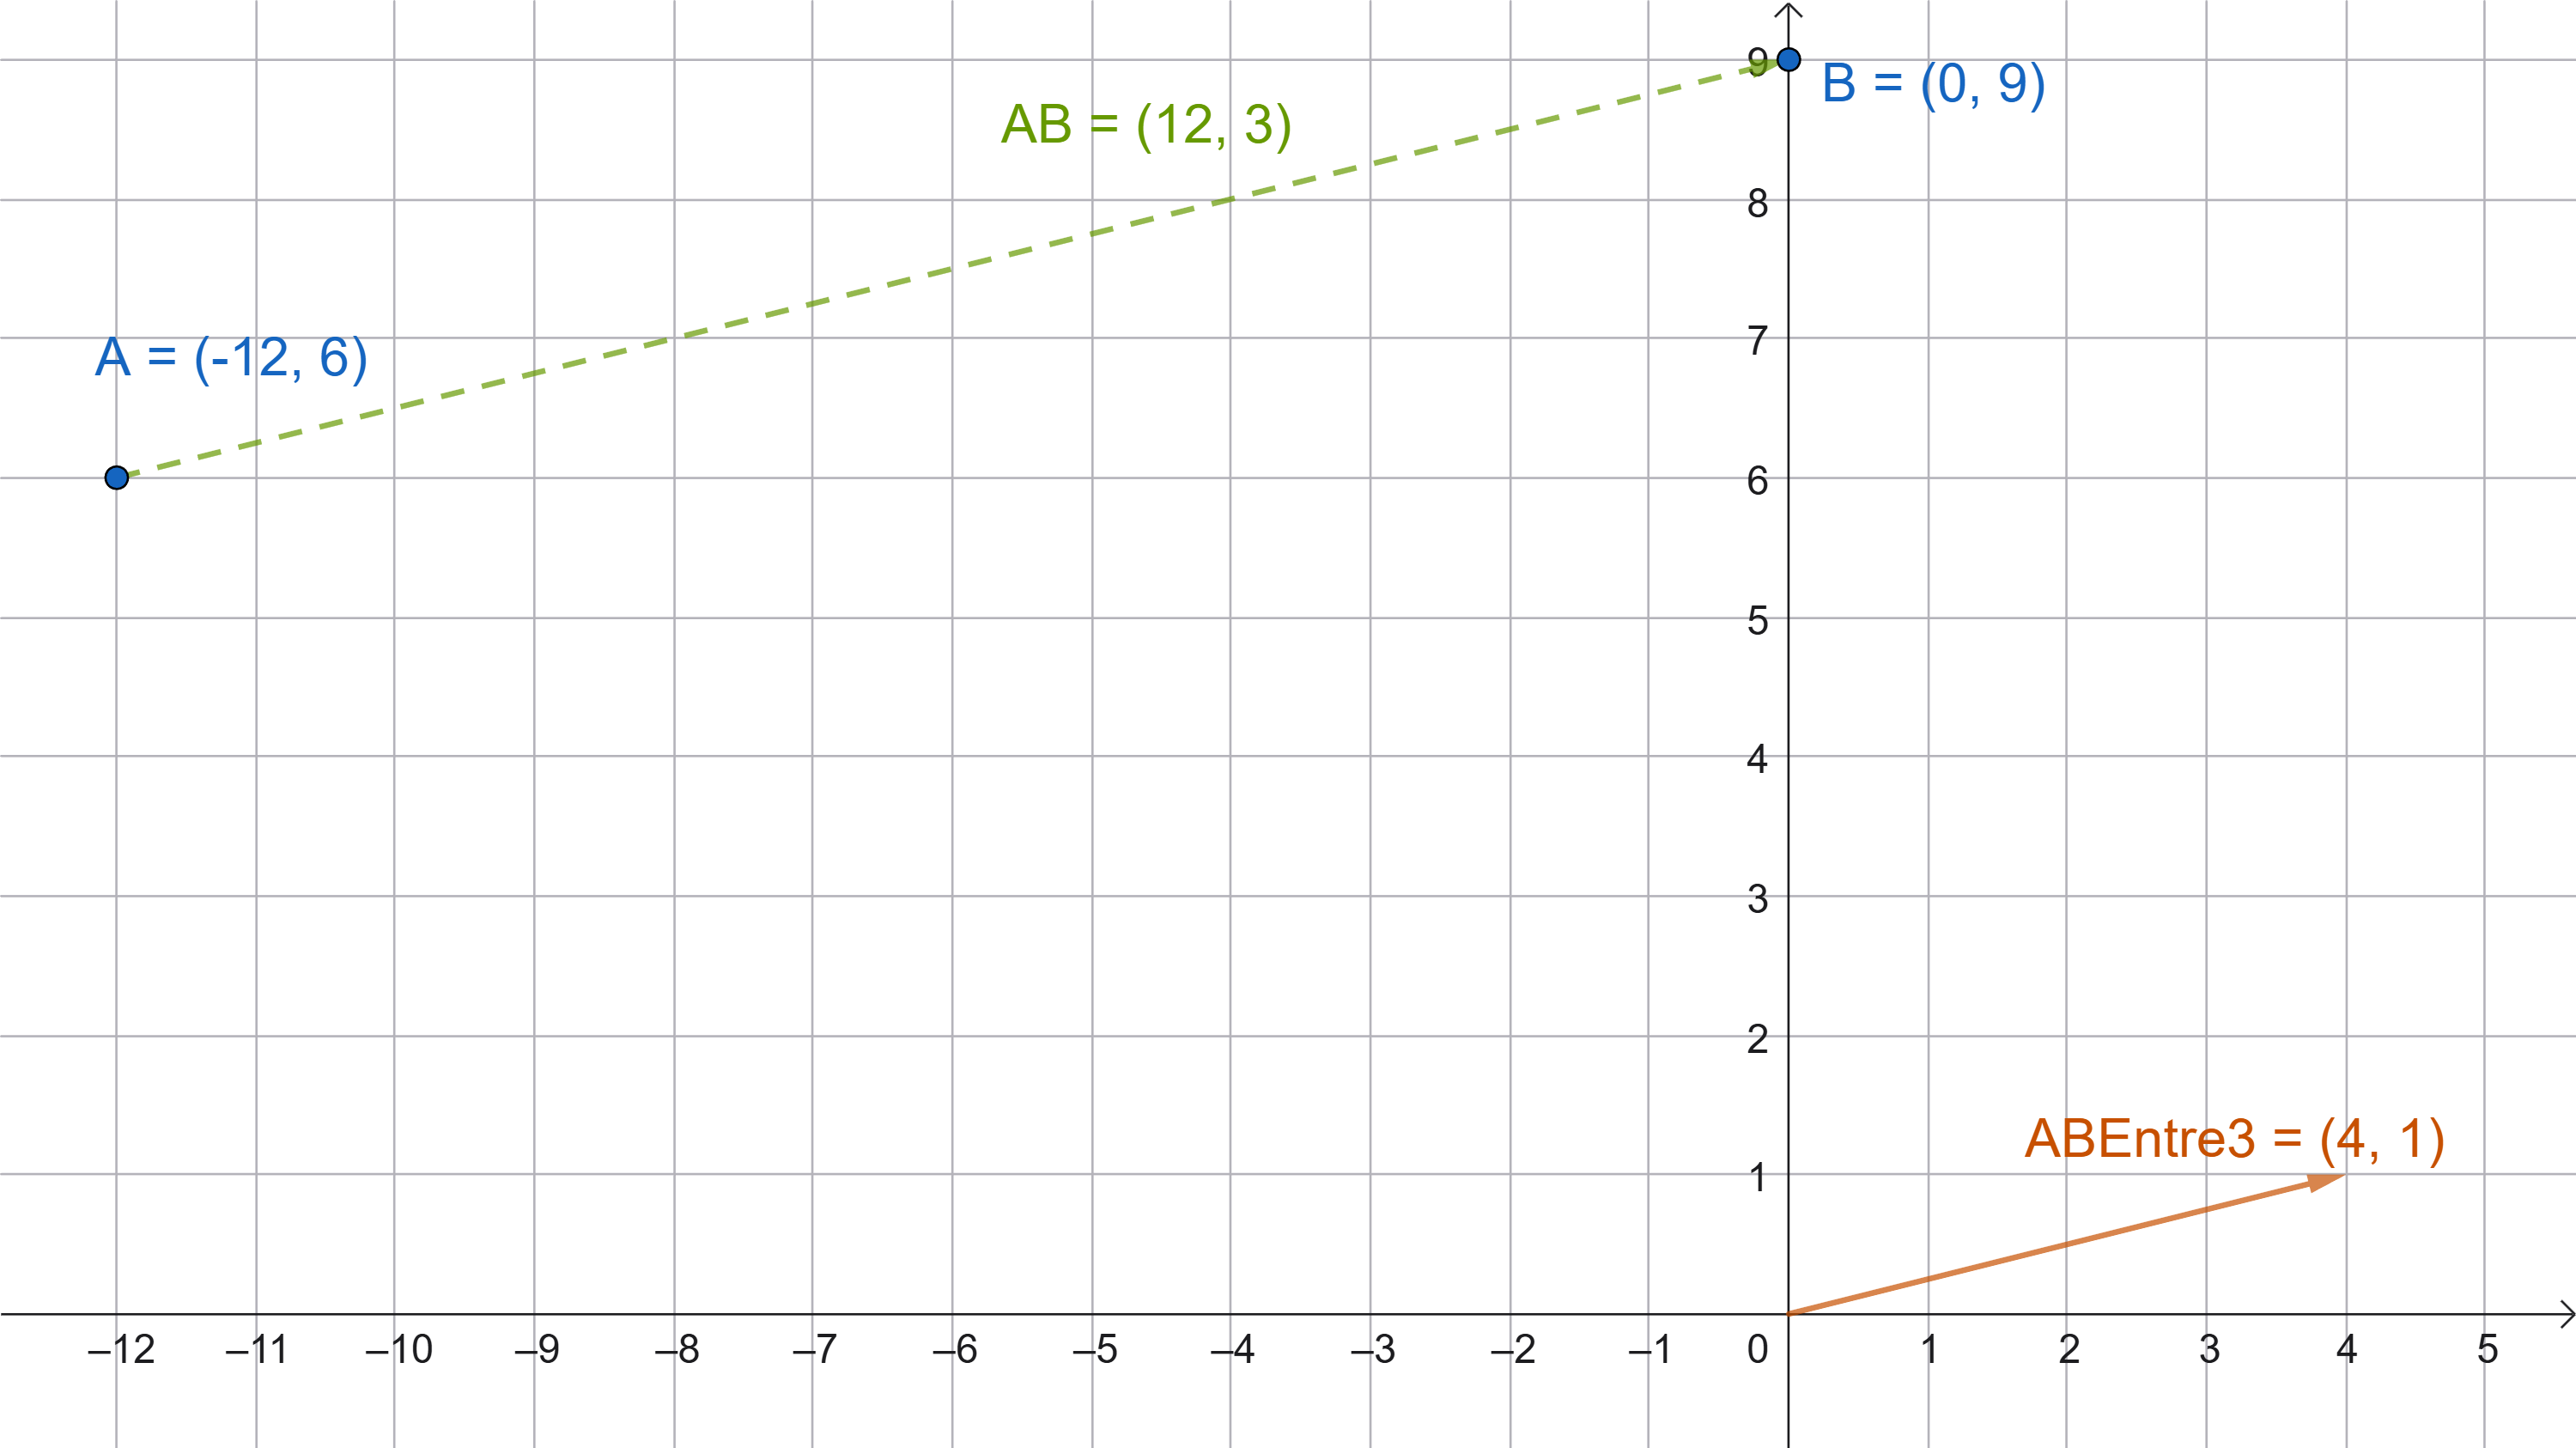
\includegraphics[width=10cm]{Vectors - 44 - Dividir punt en 3 segments_3.png}
\end{center}

\subsubsection*{4. Càlcul del primer punt ($A_1$)}
Sumem aquest vector reduït al punt inicial $A$ per trobar el primer tall.
$$ A_1 = A + \vec{v} $$
$$ A_1 = (-12, 6) + (4, 1) $$
$$ A_1 = (-12 + 4, 6 + 1) = (-8, 7) $$

El primer punt és \textbf{$A_1(-8, 7)$}.

\begin{center}
    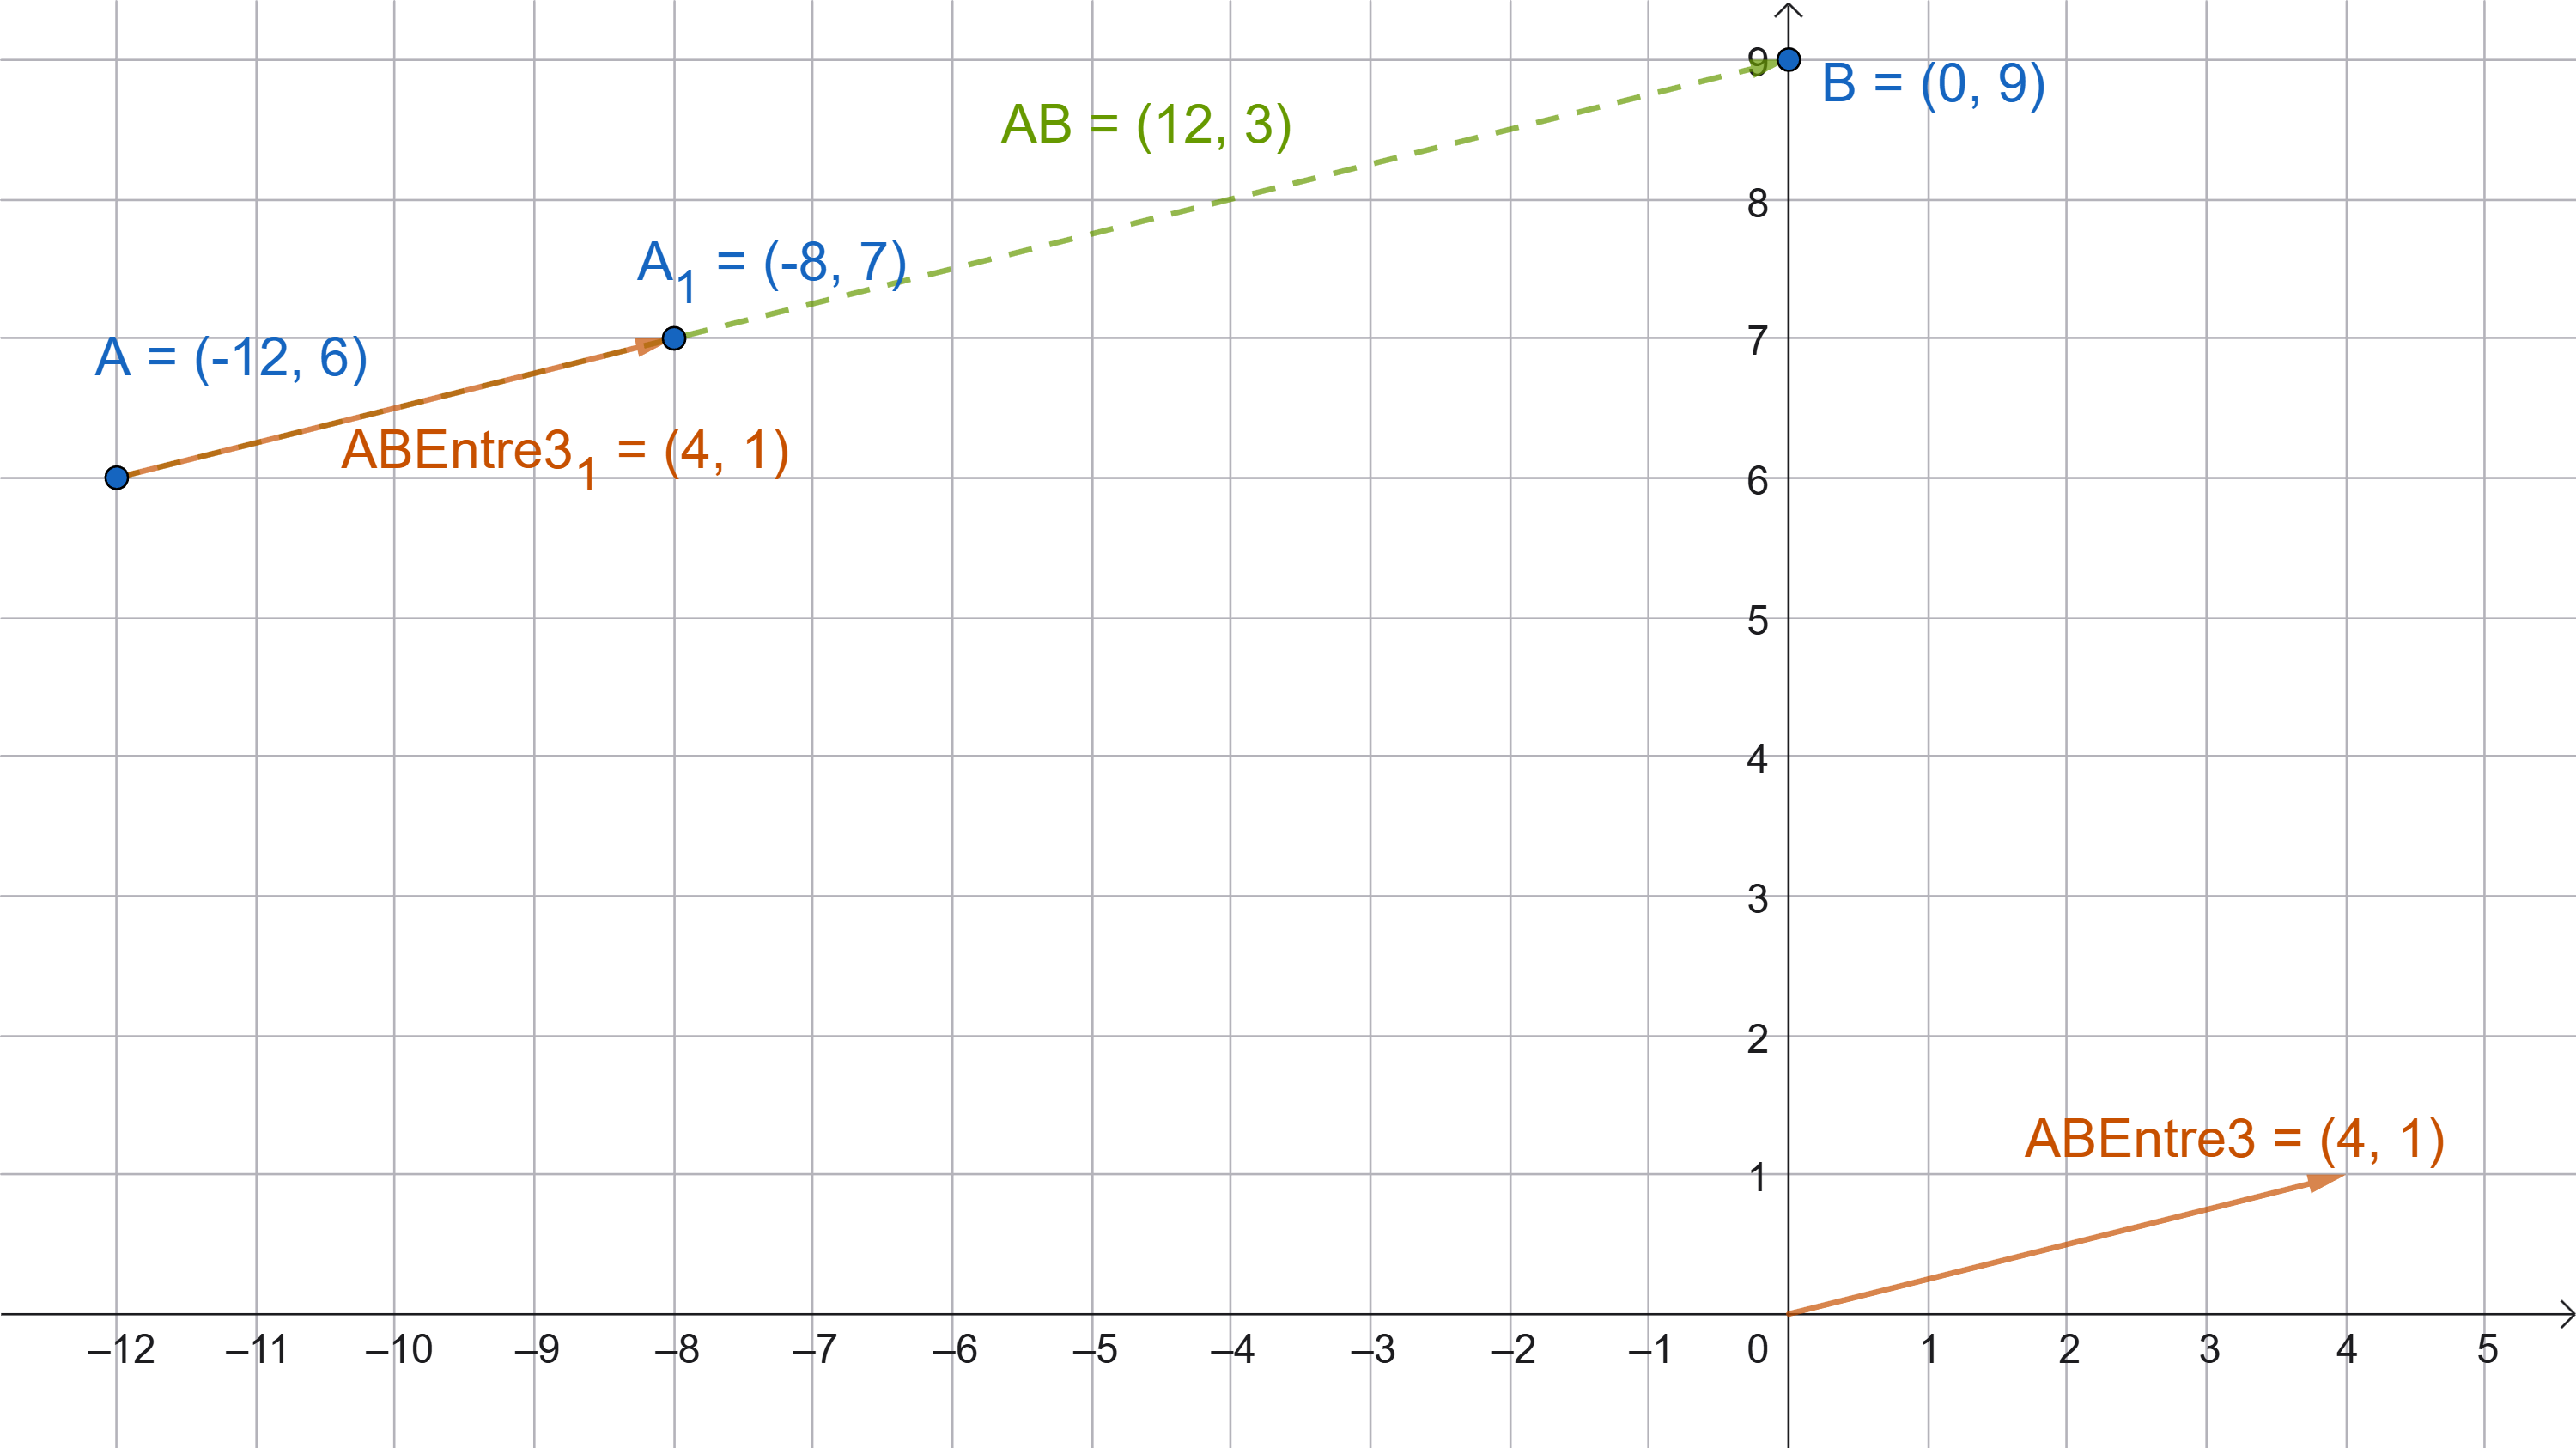
\includegraphics[width=10cm]{Vectors - 44 - Dividir punt en 3 segments_4.png}
\end{center}

\subsubsection*{5. Càlcul del segon punt ($A_2$)}
Per trobar el segon punt, podem sumar el vector $\vec{v}$ al punt $A_1$ que acabem de trobar:
$$ A_2 = A_1 + \vec{v} $$
$$ A_2 = (-8, 7) + (4, 1) $$
$$ A_2 = (-8 + 4, 7 + 1) = (-4, 8) $$

El segon punt és \textbf{$A_2(-4, 8)$}.

\begin{center}
    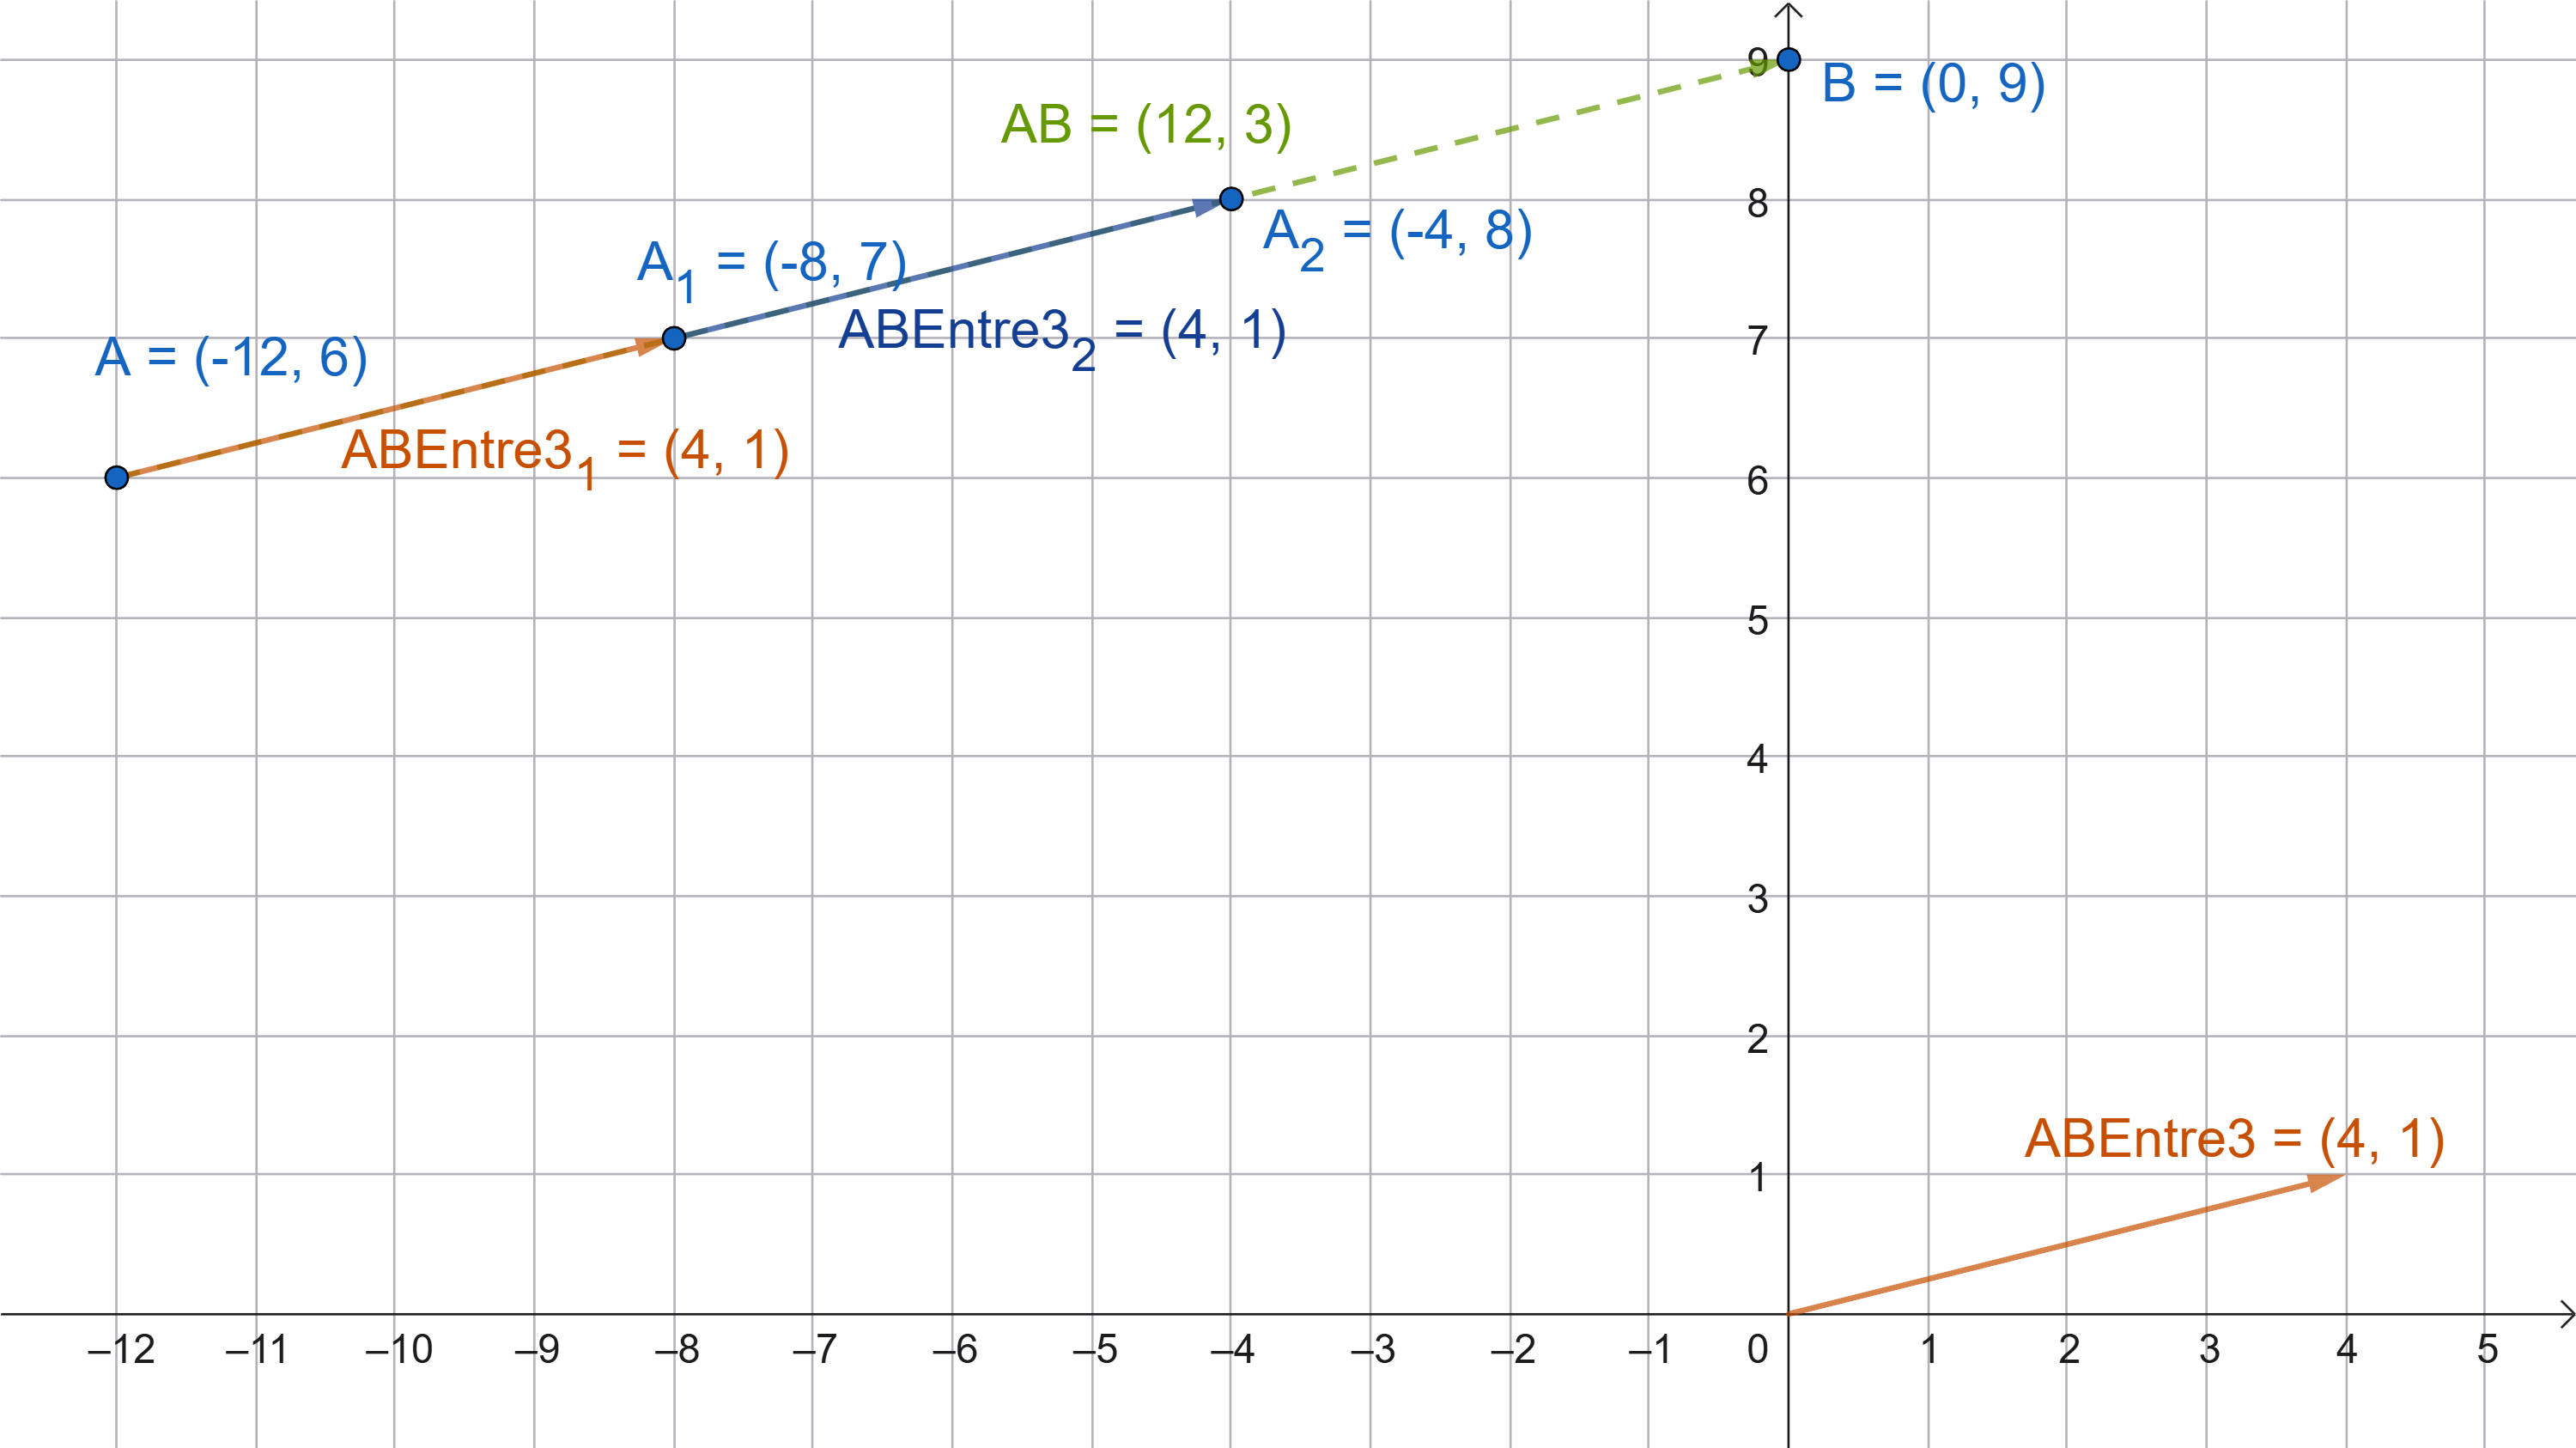
\includegraphics[width=10cm]{Vectors - 44 - Dividir punt en 3 segments_5.png}
\end{center}

\newpage

% ---------------------------------------------------------
% EXERCICI 46: BARICENTRE
% ---------------------------------------------------------

\section{Exercici 46: Baricentre d'un triangle}

\subsection*{Enunciat}
Donat el triangle format pels vèrtexs $P(3, -4)$, $Q(-2, 6)$ i $R(4, 10)$, calcula les coordenades del seu baricentre (punt $M$) utilitzant operacions amb vectors.

\vspace{0.3cm}
\noindent \textbf{Recurs interactiu:} \url{https://www.geogebra.org/calculator/xjsud8fu}

\subsection*{Resolució}

\subsubsection*{1. Identificació dels vèrtexs}
Situem els punts $P$, $Q$ i $R$ en el pla cartesià i dibuixem el triangle.

\begin{center}
    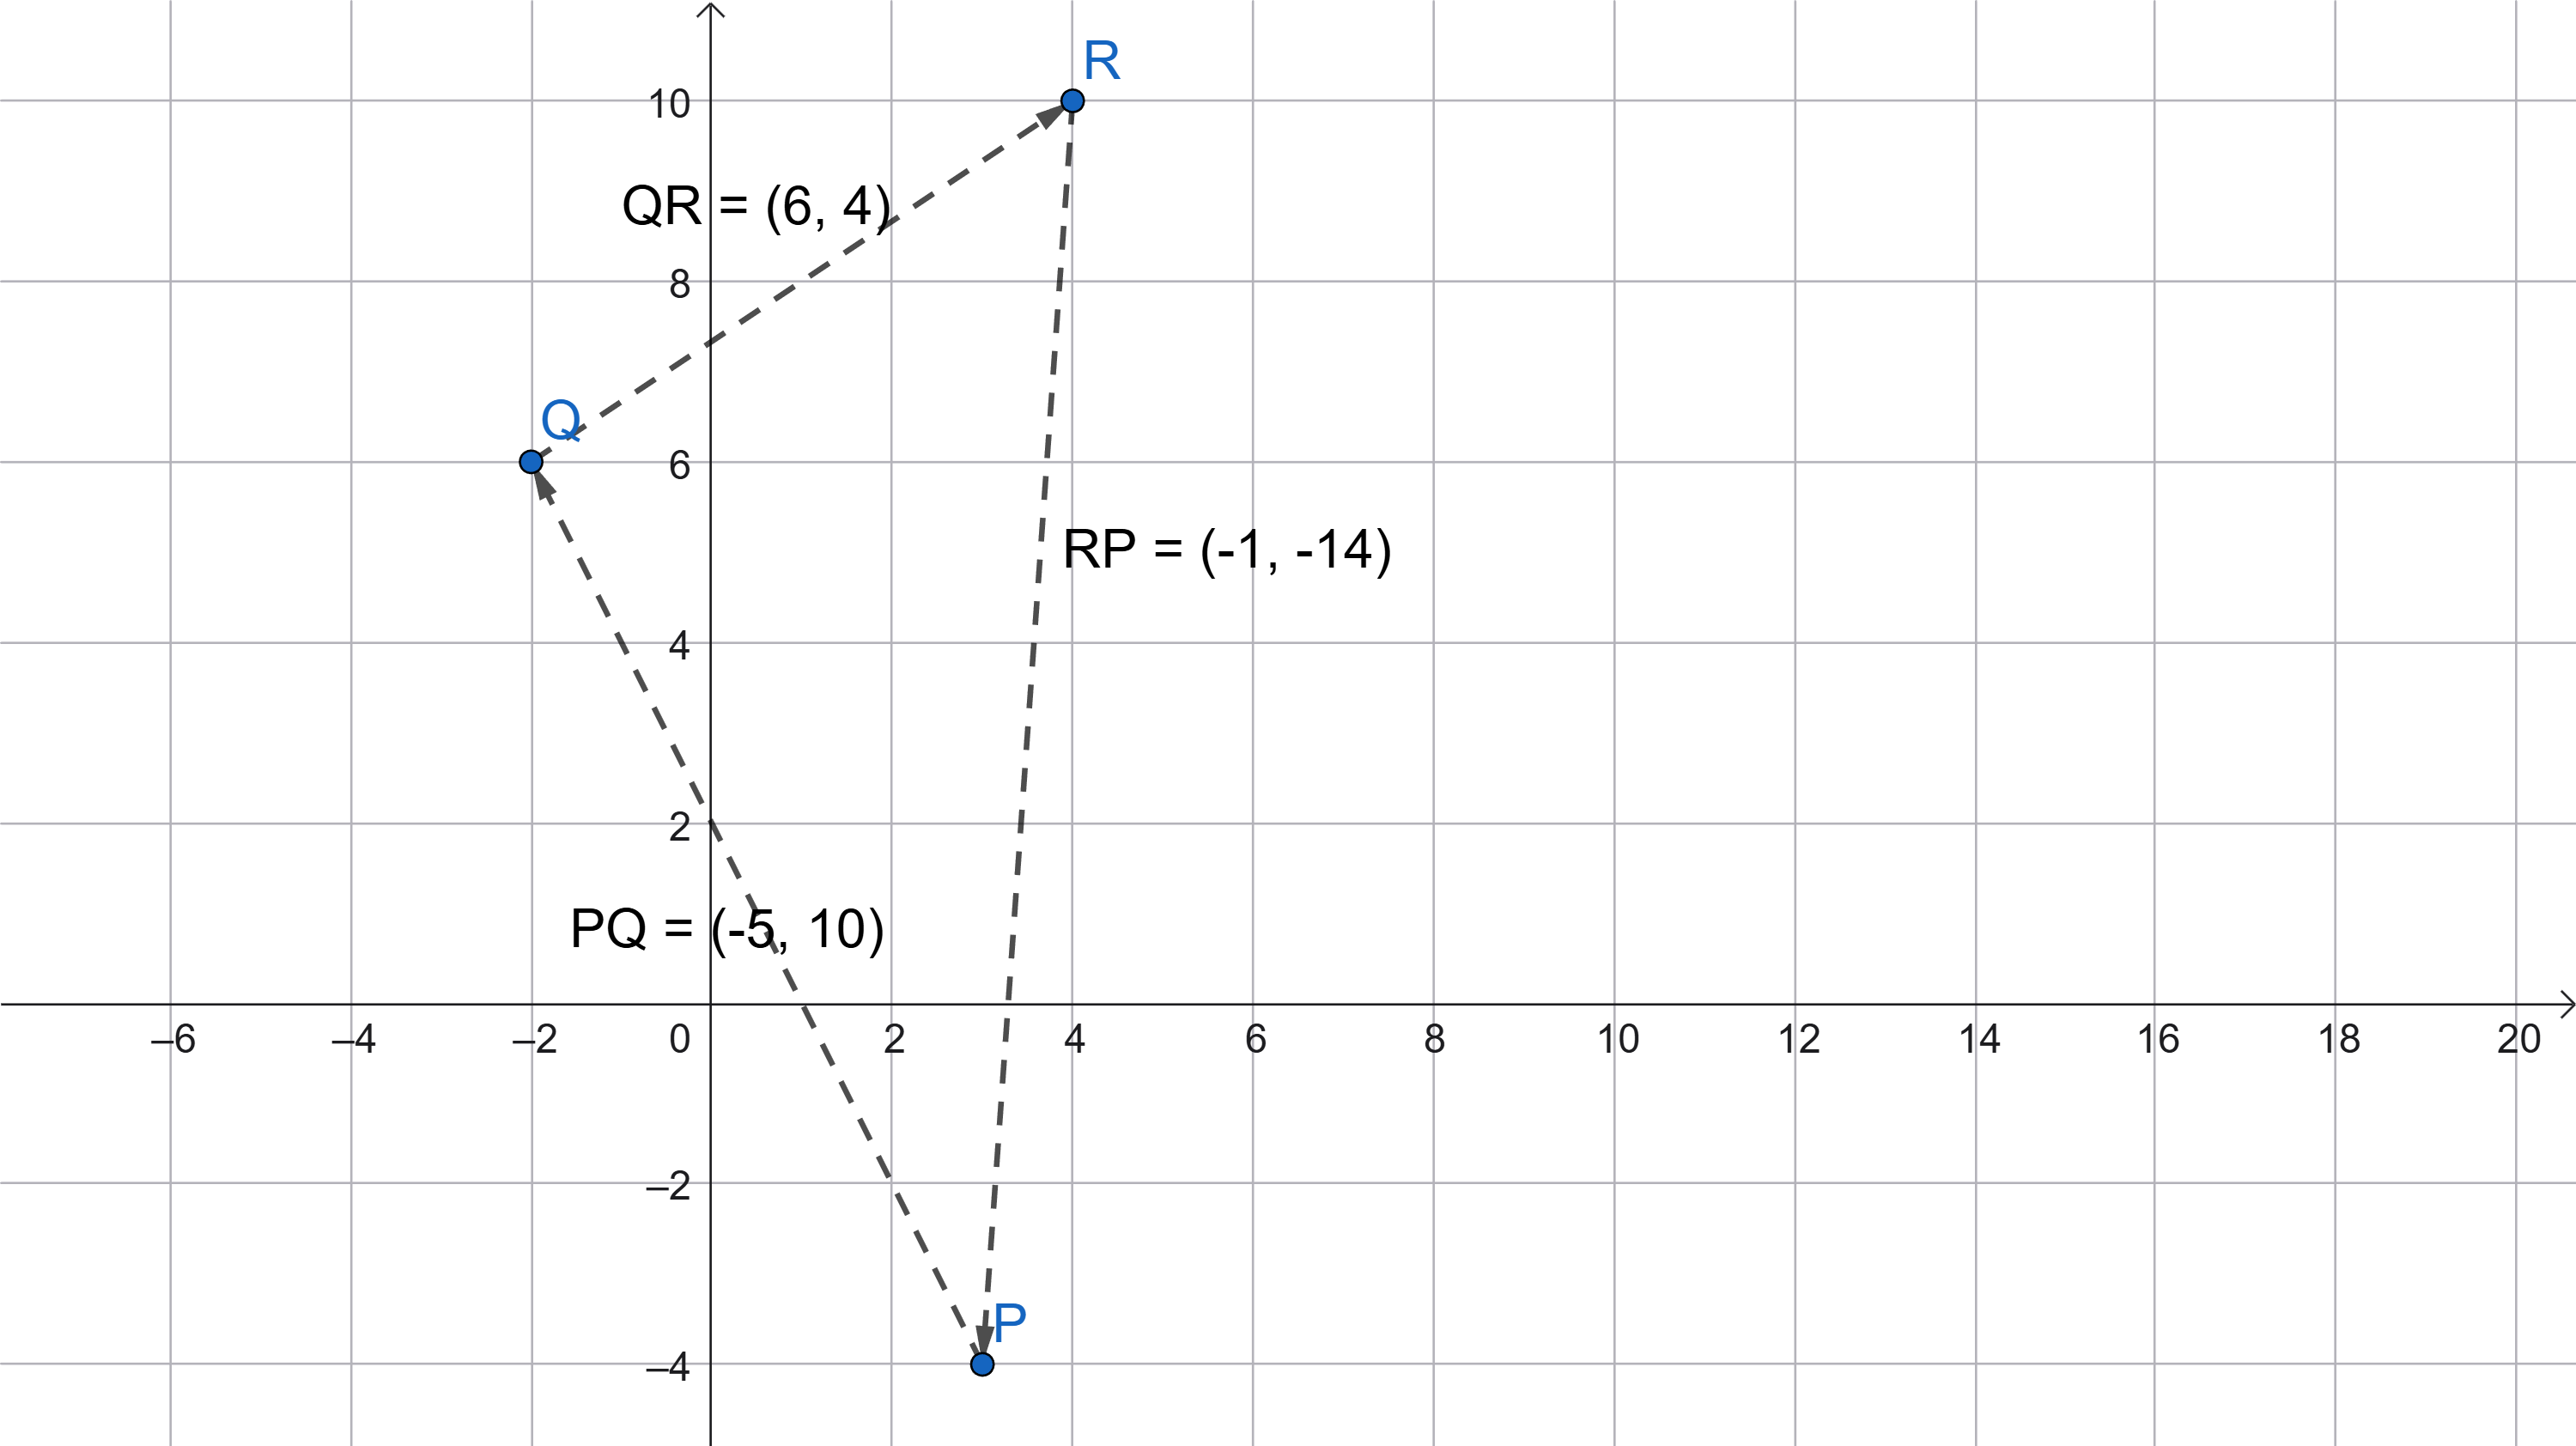
\includegraphics[width=10cm]{Vectors - 46 - Baricentre d'un triangle_1.png}
\end{center}

\subsubsection*{2. Càlcul del punt mig del costat oposat ($A$)}
Busquem el punt $A$ sobre el segment $QR$. Ho farem sumant al punt $Q$ la meitat del vector $\vec{QR}$.

$$ \vec{QR} = R - Q = (4 - (-2), 10 - 6) = (6, 4) $$

Ara, calculem el punt mig $A$:
$$ A = Q + \frac{1}{2}\vec{QR} = (-2, 6) + \frac{1}{2}(6, 4) $$
$$ A = (-2, 6) + (3, 2) = (1, 8) $$
El punt mig és \textbf{$A(1, 8)$}.

\subsubsection*{3. Càlcul del vector de la mitjana ($\vec{AP}$)}
$$ \vec{AP} = P - A = (3, -4) - (1, 8) = (2, -12) $$

\begin{center}
    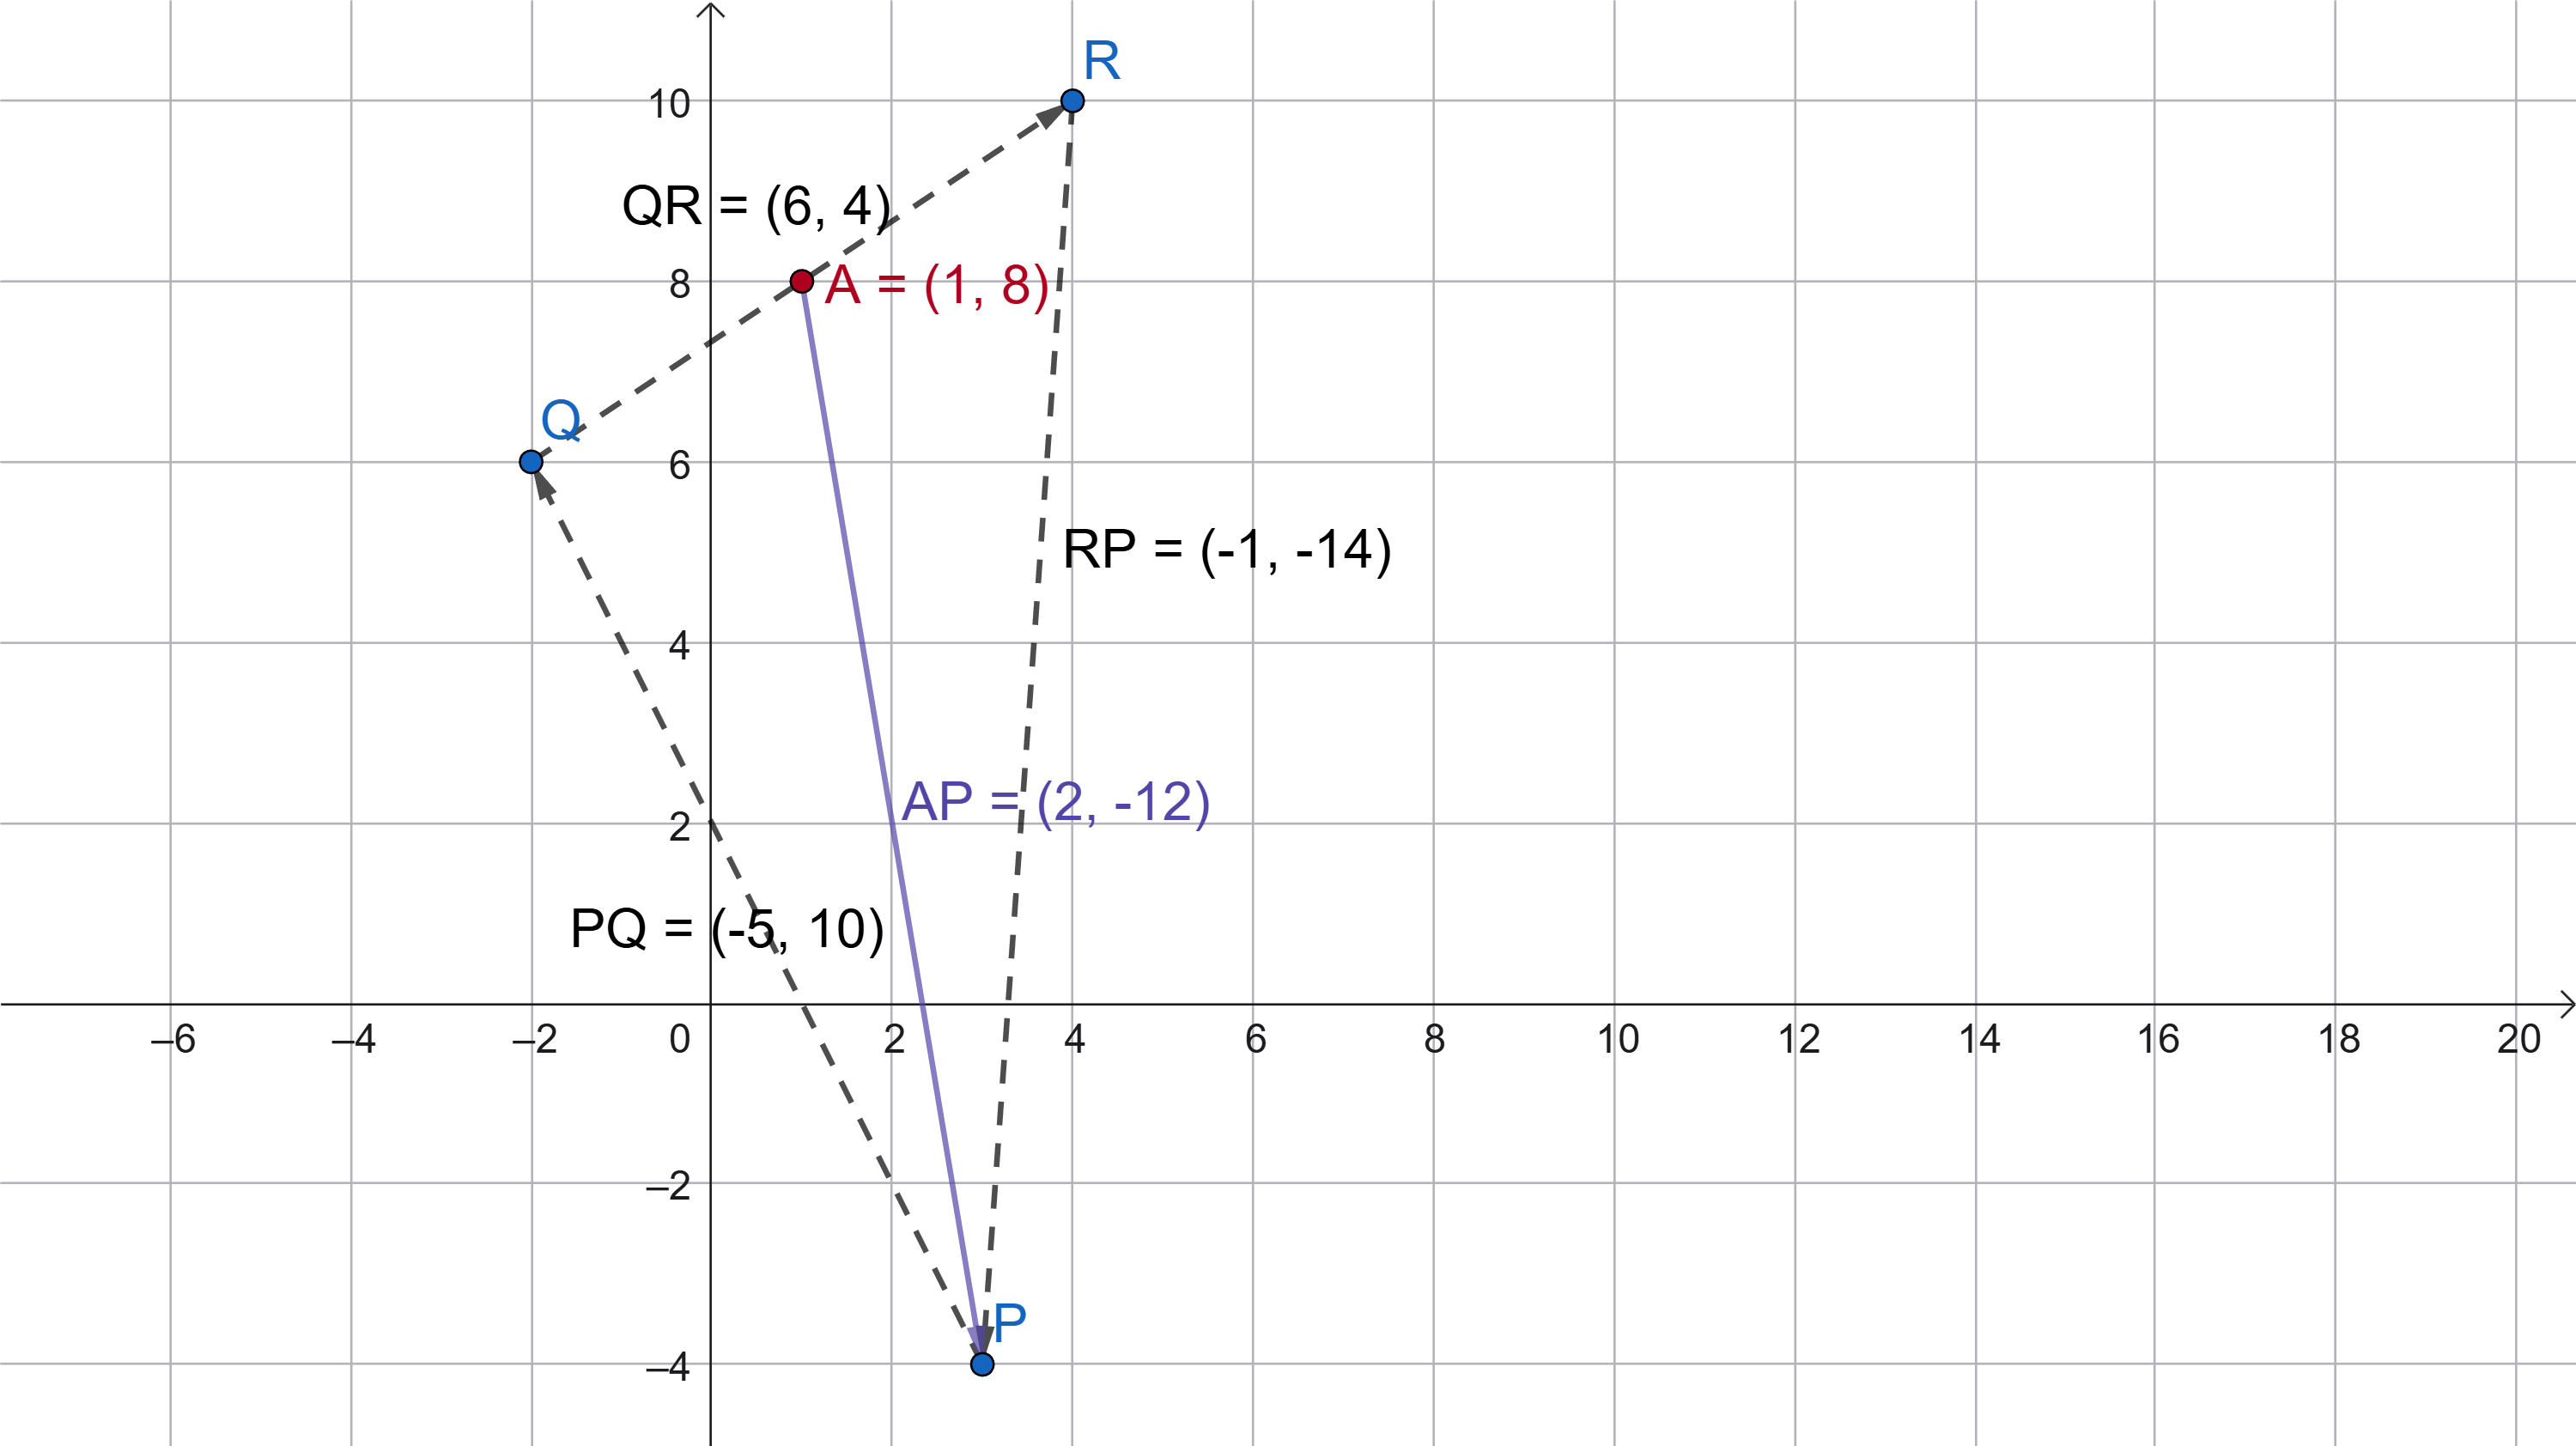
\includegraphics[width=10cm]{Vectors - 46 - Baricentre d'un triangle_2.png}
\end{center}

\subsubsection*{4. Propietat del baricentre}
El baricentre ($M$) es troba a $1/3$ de la distància de la mitjana des de $A$.
$$ \frac{1}{3}\vec{AP} = \frac{1}{3} \cdot (2, -12) = \left( \frac{2}{3}, -4 \right) $$

\begin{center}
    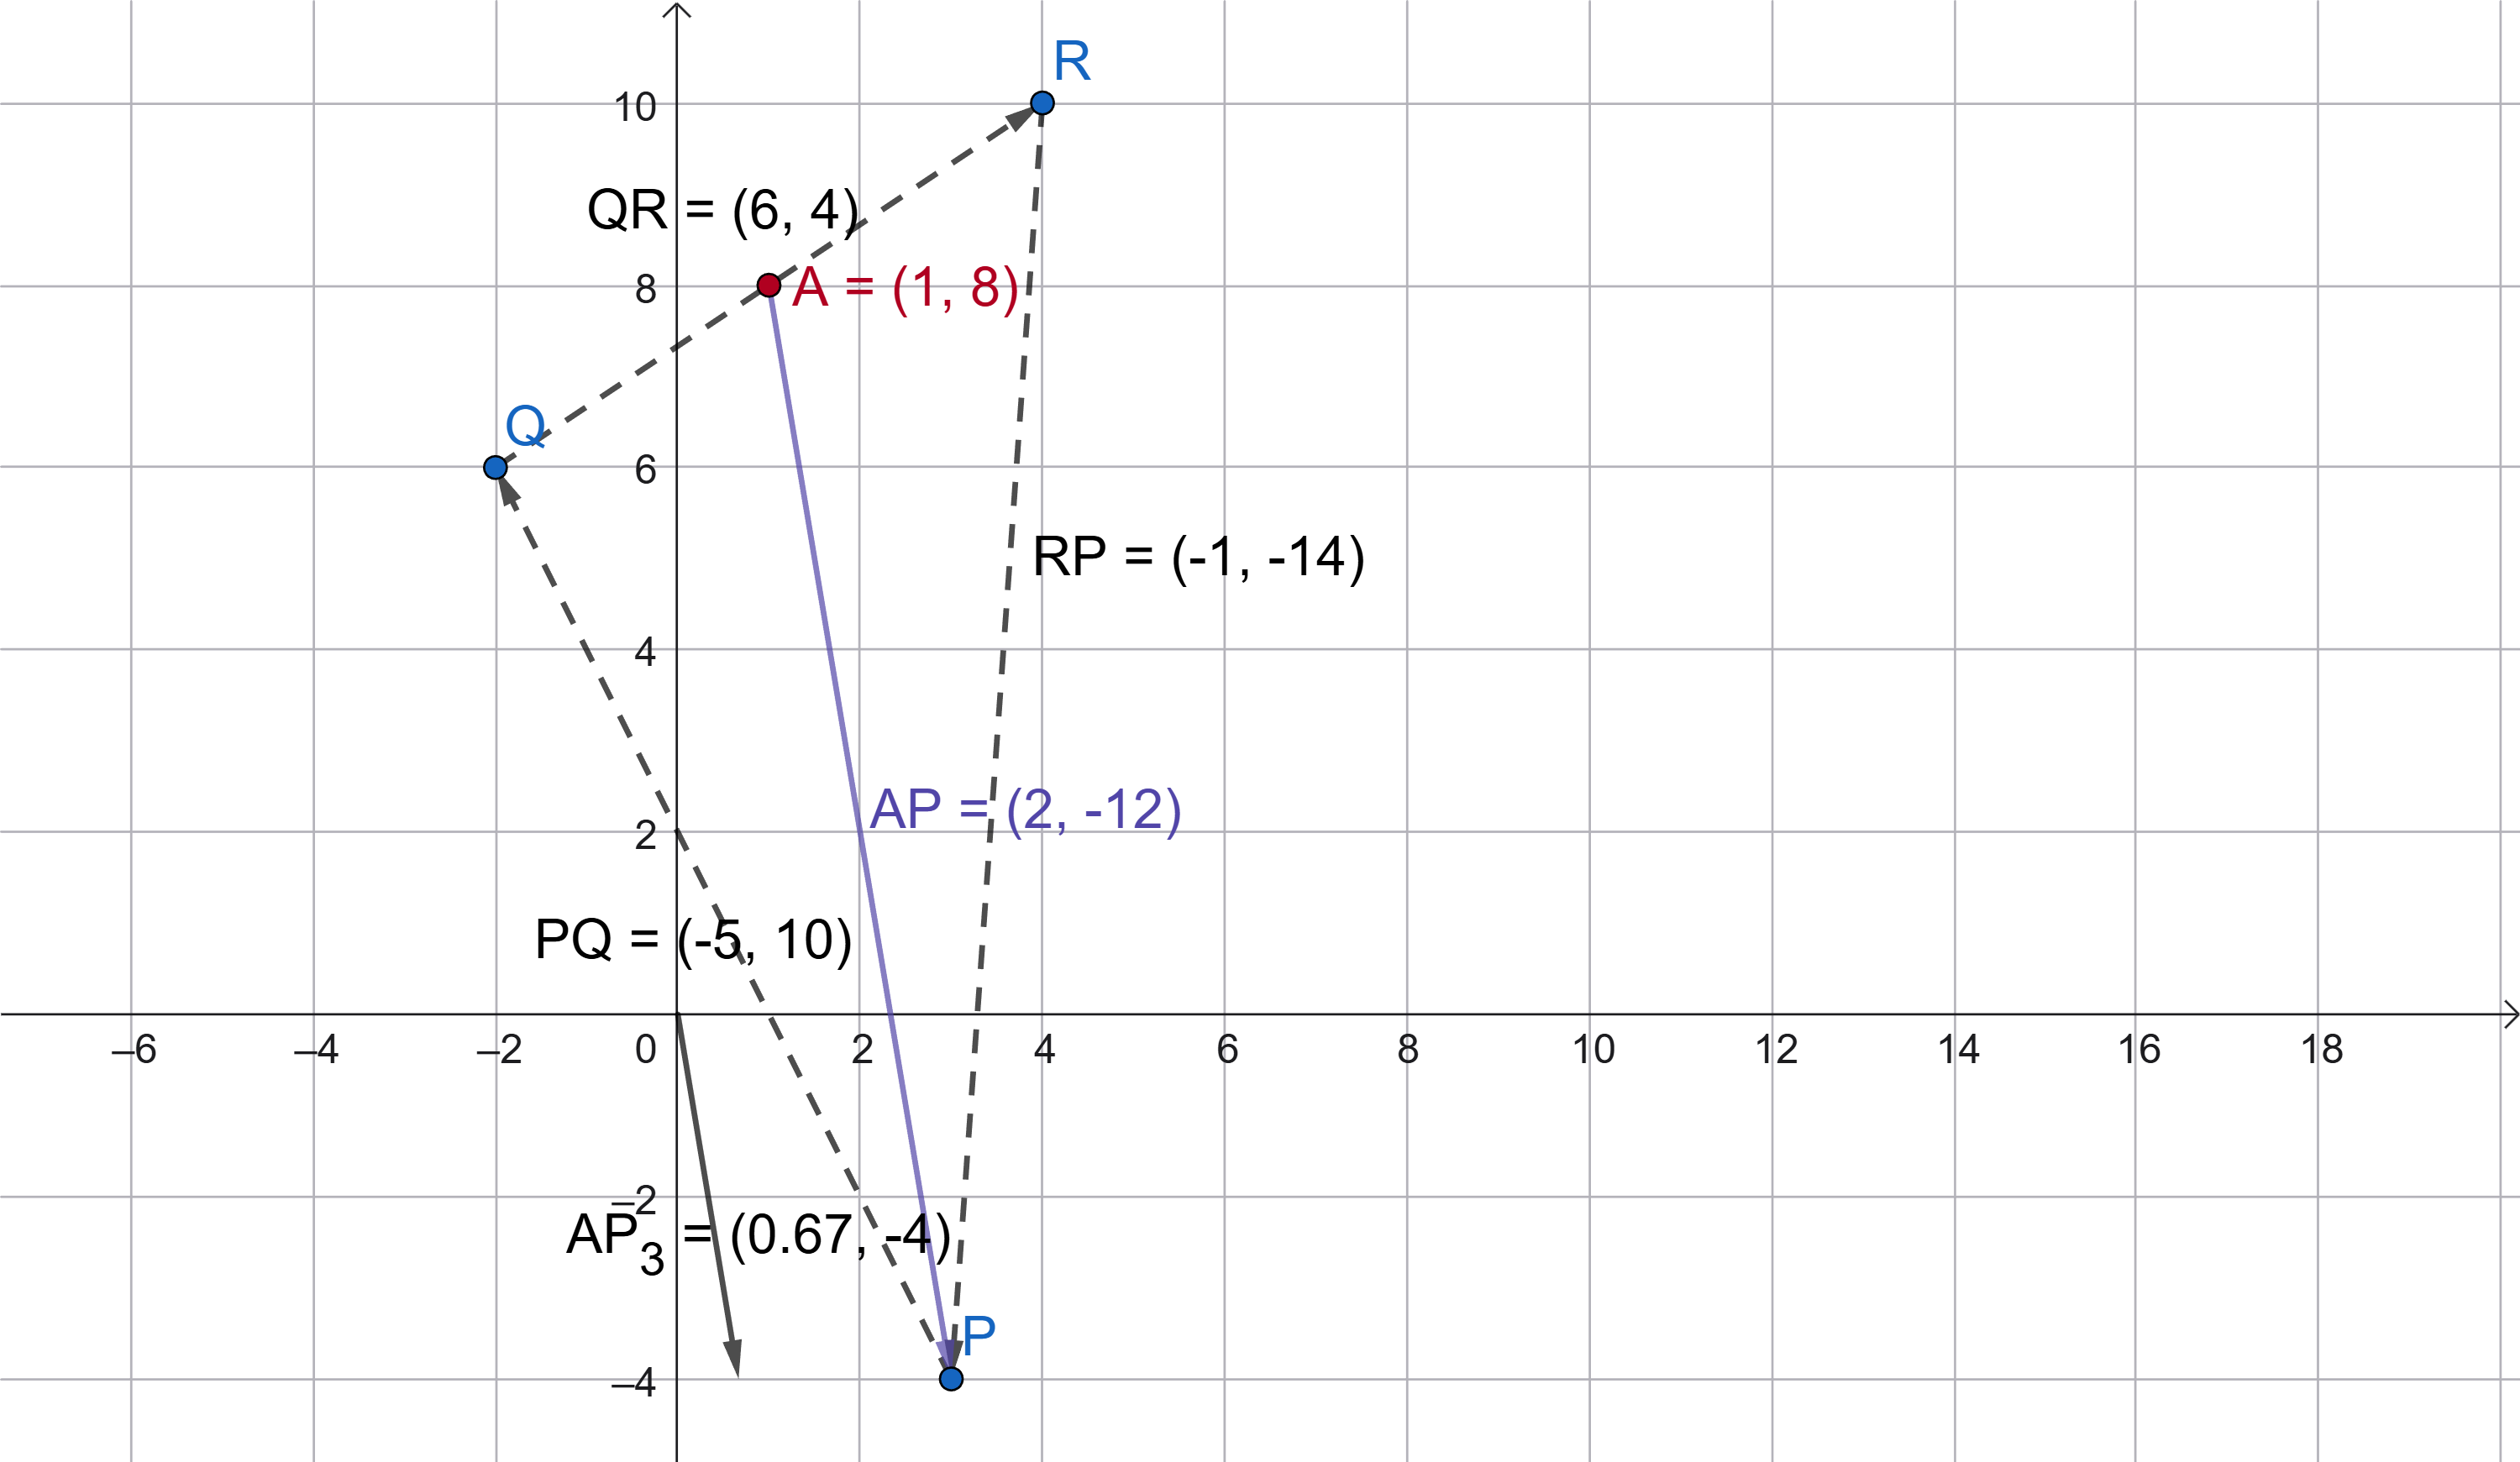
\includegraphics[width=10cm]{Vectors - 46 - Baricentre d'un triangle_3.png}
\end{center}

\subsubsection*{5. Càlcul final del Baricentre ($M$)}
$$ M = A + \frac{1}{3}\vec{AP} = (1, 8) + \left( \frac{2}{3}, -4 \right) $$
$$ x_M = 1 + \frac{2}{3} = \frac{5}{3}, \quad y_M = 8 - 4 = 4 $$

$$ \textbf{M = \left( \frac{5}{3}, 4 \right)} $$

\begin{center}
    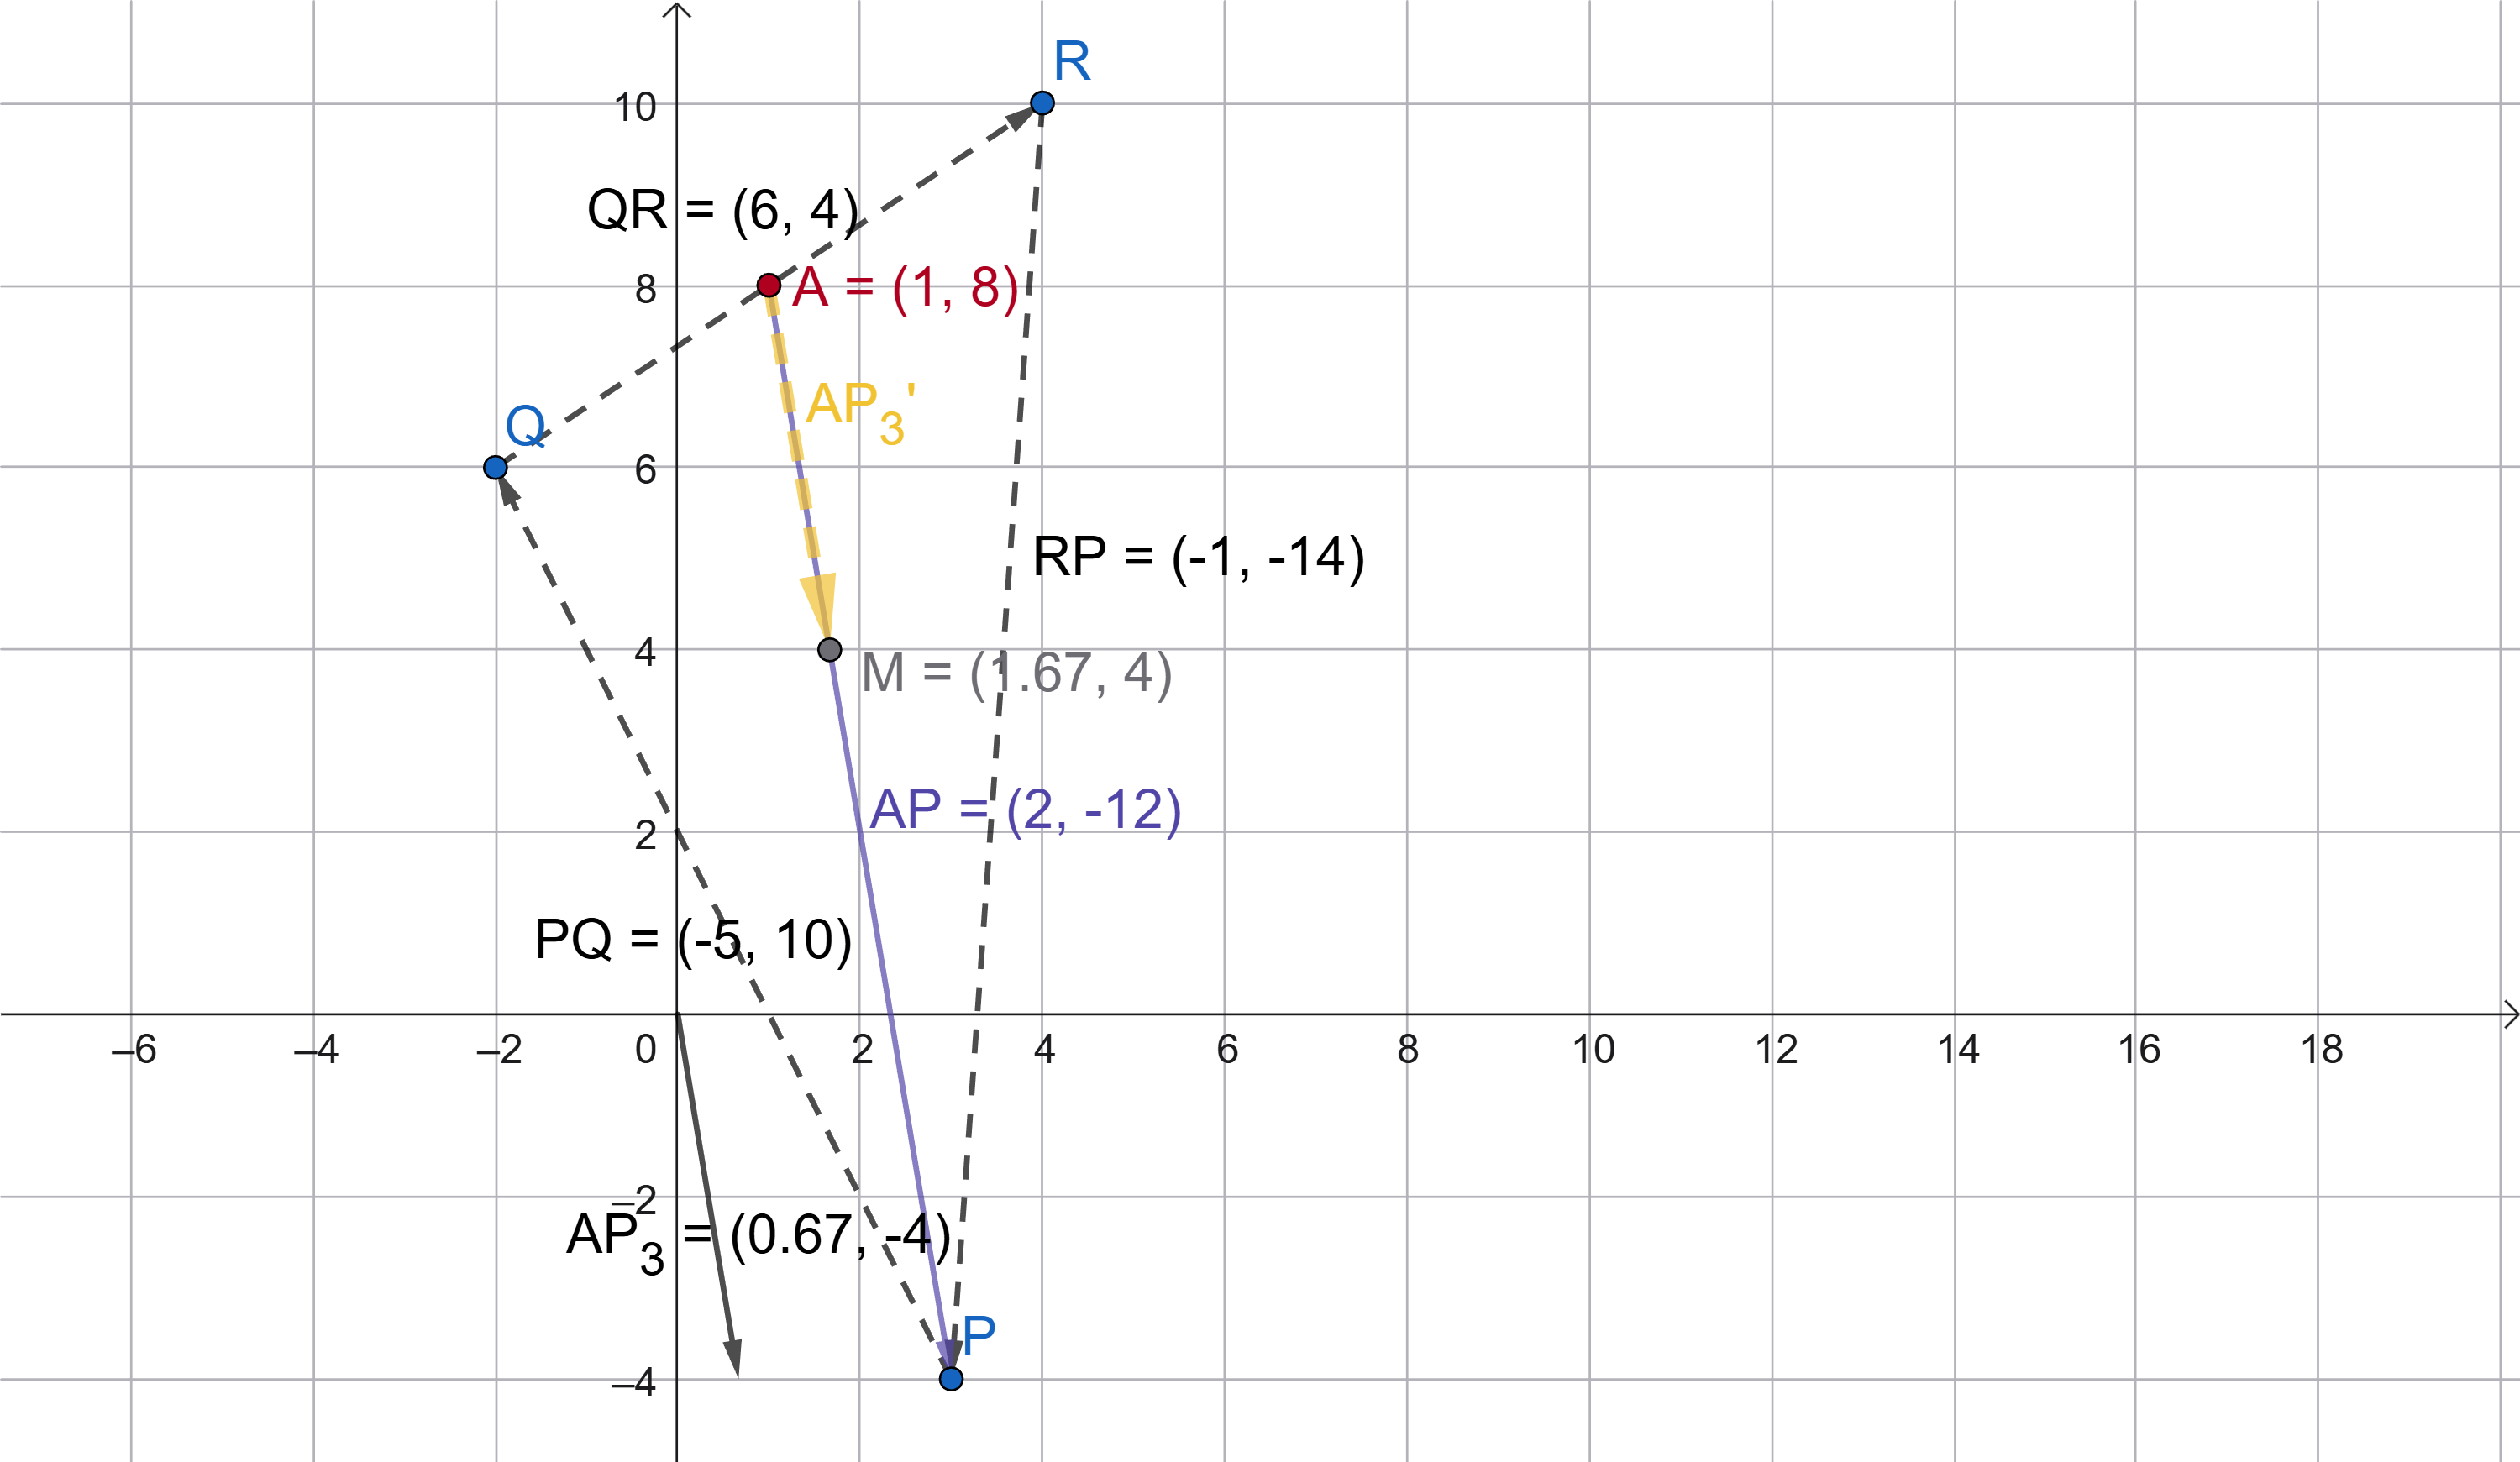
\includegraphics[width=10cm]{Vectors - 46 - Baricentre d'un triangle_4.png}
\end{center}

\end{document}